\newpage
\section{BA ĐƯỜNG CONIC TRONG MẶT PHẲNG TỌA ĐỘ}
\subsection{Trọng tâm kiến thức}
\subsubsection{Elip}
	\begin{khung4}{Định nghĩa}
		\immini{
			Cho hai điểm cố định $F_1$, $F_2$ và độ dài $F_1F_2=2c>0$.\\
			\textbf{Đường elip $(E)$} hay elip $(E)$ là tập hợp các điểm $M$ trong mặt phẳng sao cho $MF_1+MF_2=2a$, với $a$ là số thực dương cho trước và $a>c$.\\
			Ta viết gọn như sau
			$$(E)= \{M\mid MF_1+MF_2=2a\,,\text{với } a>c\}.$$
			Hai điểm $F_1$ và $F_2$ gọi là hai \textbf{tiêu điểm} của elip $(E)$.\\
			Độ dài $F_1F_2=2c$ gọi là \textbf{tiêu cự} của elip.
		}{
			\begin{tikzpicture}[scale=0.6, font=\footnotesize, line join=round, line cap=round, >=stealth]
				\def\a{2.4};
				\def\b{1.6};
				\pgfmathsetmacro\c{sqrt((\a)^2-(\b)^2)};
				\draw[name path=e] (0,0) ellipse (\a cm and \b cm);
				\path
				($(0,0) + (60:{\a} and {\b})$) coordinate (M)
				(-\c,0) coordinate (F_1)
				(\c,0) coordinate (F_2)
				($(M)+(108:0.4)$) coordinate (A)
				($(M)+(140:0.4)$) coordinate (B)
				($(A)+(124:2)$) coordinate (D)
				($(B)+(D)-(A)$) coordinate (C)
				($(C)!0.5!(D)$) coordinate (E)
				;
				\foreach \i/\j in {M/above right,F_1/below,F_2/below}
				\draw[fill=black] (\i) circle(1pt) node[\j]{$\i$};
				\draw (M)--(F_1)--(F_2)--(M);
				%cây viết
				\draw (A)--(M)--(B);
				\fill[gray,draw=black] (A)--(B)--(C)--(D)--(A);
				\fill[rotate=34,white,draw=black] (D) arc(0:360:0.11 and 0.05);
				\fill[rotate=34,black] (E) ellipse (0.05 and 0.025);
			\end{tikzpicture}
		}
	\end{khung4}
	\begin{khung4}{Phương trình chính tắc}
		\immini{
			Chọn hệ trục toạ độ $Oxy$ như hình vẽ bên. Khi đó phương trình chính tắc của  đường elip $(E)$ có dạng là	
			$$\dfrac{x^2}{a^2}+\dfrac{y^2}{b^2}=1\,,\heva{&a>b>0\\
			&c^2=a^2-b^2.}$$ 
			}{
			\begin{tikzpicture}[scale=0.6, font=\footnotesize, line join=round, line cap=round, >=stealth]
				\def\a{2.4};
				\def\b{1.6};
				\pgfmathsetmacro\c{sqrt((\a)^2-(\b)^2)};
				\draw[->] ($(-{\a},0)-(1,0)$)--($({\a},0)+(1,0)$) node[above]{$x$};
				\draw[->] ($(0,-{\b})-(0,1)$)--($(0,{\b})+(0,1)$) node[left]{$y$};
				\draw[name path=e] (0,0) ellipse (\a cm and \b cm);
				\path
				(0,0) coordinate (O)
				($(0,0) + (55:{\a} and {\b})$) coordinate (M)
				(-\c,0) coordinate (F_1)
				(\c,0) coordinate (F_2)
				(-\a,0) coordinate (A_1)
				(\a,0) coordinate (A_2)
				(0,-\b) coordinate (B_1)
				(0,\b) coordinate (B_2)
				;
				\foreach \i/\j in {F_1/below,F_2/below,O/below left,A_1/below left,A_2/below right,B_1/below right,B_2/above right}
				\draw[fill=black] (\i) circle(1pt) node[\j]{$\i$};
				\draw[fill=black] (M) circle(1pt) node[above right]{$M(x;y)$};
				\draw (M)--(F_1) (F_2)--(M);
			\end{tikzpicture}
		}
	\end{khung4}
	\begin{khung4}{Các yếu tố của elip}
		Cho elip $(E)$ có phương trình chính tắc là $$\dfrac{x^2}{a^2}+\dfrac{y^2}{b^2}=1\,,\heva{&a>b>0\\
			&c^2=a^2-b^2.}$$ 
		Khi đó:
		\begin{itemize}
			\item $(E)$ cắt $Ox$ tại hai điểm $A_1(-a;0)$, $A_2(a;0)$ và cắt $Oy$ tại hai điểm $B_1(0;-b)$, $B_2(0;b)$ và các điểm $A_1$, $A_2$, $B_1$, $B_2$ được gọi là các \textbf{đỉnh} của elip.
			\item Đoạn thẳng $A_1A_2=2a$ gọi là \textbf{ độ dài trục lớn}, đoạn thẳng $B_1B_2=2b$ gọi là \textbf{ độ dài trục nhỏ} của elip.
			\item Hai \textbf{tiêu điểm} của elip là $F_1(-c;0)$ và $F_2(c;0)$.
			\item Độ dài $F_1F_2=2c$ gọi là \textbf{tiêu cự} của elip.
			\item Với điểm $M(x;y)\in (E)$ thì $\dfrac{x^2}{a^2}+\dfrac{y^2}{b^2}=1$ và $|x|\le a$, $|y|\le b$.
			\item Giao điểm $O$ của hai trục gọi là \textbf{tâm đối xứng} của elip.
			\item Hai trục $Ox$, $Oy$ là hai \textbf{trục đối xứng} của elip.
		\end{itemize}
	\end{khung4}

%Hypebol
\subsubsection{Hypebol}
\begin{khung4}{Định nghĩa}
	\immini{
		Cho hai điểm cố định $F_1$, $F_2$ và độ dài $F_1F_2=2c>0$.\\
		\textbf{Đường hypebol $(H)$} hay hypebol $(H)$ là tập hợp các điểm $M$ trong mặt phẳng sao cho $\left|MF_1-MF_2\right|=2a$, với $a$ là số thực dương cho trước và $a<c$.\\
		Ta viết gọn như sau
		$$(H)= \{M\mid \left|MF_1-MF_2\right|=2a\,,\text{với } a<c\}.$$
		Hai điểm $F_1$ và $F_2$ gọi là hai \textbf{tiêu điểm} của hypebol $(H)$.\\
		Độ dài $F_1F_2=2c$ gọi là \textbf{tiêu cự} của hypebol.
	}{
		\begin{tikzpicture}[scale=0.7, font=\footnotesize, line join=round, line cap=round, >=stealth]
			\def\a{1.2};
			\def\b{1};
			\pgfmathsetmacro\c{sqrt((\a)^2+(\b)^2)};
			\draw[name path=h1,smooth, samples=200, domain=\a:2.5] plot (\x,{((\b)/(\a))*sqrt((\x)^2-(\a)^2)});
			\draw[yscale=-1,name path=h2,smooth, samples=200, domain=\a:2.5] plot (\x,{((\b)/(\a))*sqrt((\x)^2-(\a)^2)});
			\draw[xscale=-1,name path=h2,smooth, samples=200, domain=\a:2.5] plot (\x,{((\b)/(\a))*sqrt((\x)^2-(\a)^2)});
			\draw[xscale=-1,yscale=-1,name path=h2,smooth, samples=200, domain=\a:2.5] plot (\x,{((\b)/(\a))*sqrt((\x)^2-(\a)^2)});
			\def\xm{2};
			\pgfmathsetmacro\ym{((\b)/(\a))*sqrt((\xm)^2-(\a)^2)};
			\path
			(0,0) coordinate (O)
			(-\c,0) coordinate (F_1)
			(\c,0) coordinate (F_2)
			(-\a,0) coordinate (A_1)
			(\a,0) coordinate (A_2)
			(\xm,\ym) coordinate (M)
			;
			\draw[fill=black] (F_1) circle(1pt) node[below]{$F_1$};
			\draw[fill=black] (F_2) circle(1pt) node[below]{$F_2$};
			\draw[fill=black] (M) circle(1pt) node[right]{$M(x;y)$};
			\draw (F_1)--(M)--(F_2)--(F_1);
		\end{tikzpicture}
	}
\end{khung4}
\begin{khung4}{Phương trình chính tắc}
	\immini{
		Chọn hệ trục toạ độ $Oxy$ như hình vẽ bên. Khi đó phương trình chính tắc của  đường hypebol $(H)$ có dạng là	
		$$\dfrac{x^2}{a^2}-\dfrac{y^2}{b^2}=1\,,\heva{&a,b>0\\
			&c^2=a^2+b^2.}$$ 
	}{
		\begin{tikzpicture}[scale=0.7, font=\footnotesize, line join=round, line cap=round, >=stealth]
			\def\a{1.2};
			\def\b{1};
			\pgfmathsetmacro\c{sqrt((\a)^2+(\b)^2)};
			\draw[->] ($(-{\a},0)-(1.5,0)$)--($({\a},0)+(1.5,0)$) node[above]{$x$};
			\draw[->] ($(0,-{\b})-(0,1)$)--($(0,{\b})+(0,1)$) node[left]{$y$};
			\draw[name path=h1,smooth, samples=200, domain=\a:2.5] plot (\x,{((\b)/(\a))*sqrt((\x)^2-(\a)^2)});
			\draw[yscale=-1,name path=h2,smooth, samples=200, domain=\a:2.5] plot (\x,{((\b)/(\a))*sqrt((\x)^2-(\a)^2)});
			\draw[xscale=-1,name path=h2,smooth, samples=200, domain=\a:2.5] plot (\x,{((\b)/(\a))*sqrt((\x)^2-(\a)^2)});
			\draw[xscale=-1,yscale=-1,name path=h2,smooth, samples=200, domain=\a:2.5] plot (\x,{((\b)/(\a))*sqrt((\x)^2-(\a)^2)});
			\def\xm{2};
			\pgfmathsetmacro\ym{((\b)/(\a))*sqrt((\xm)^2-(\a)^2)};
			\path
			(0,0) coordinate (O)
			(-\c,0) coordinate (F_1)
			(\c,0) coordinate (F_2)
			(-\a,0) coordinate (A_1)
			(\a,0) coordinate (A_2)
			(\xm,\ym) coordinate (M)
			;
			\draw[fill=black] (O) circle(1pt) node[below left]{$O$};
			\draw[fill=black] (F_1) circle(1pt) node[below]{$F_1$};
			\draw[fill=black] (F_2) circle(1pt) node[below]{$F_2$};
			\draw[fill=black] (M) circle(1pt) node[right]{$M(x;y)$};
			\draw (F_1)--(M)--(F_2);
		\end{tikzpicture}
	}
\end{khung4}
\begin{khung4}{Các yếu tố của hypebol}
	Cho hypebol $(H)$ có phương trình chính tắc là $$\dfrac{x^2}{a^2}-\dfrac{y^2}{b^2}=1\,,\heva{&a,b>0\\
		&c^2=a^2+b^2.}$$ 
	Khi đó:
	\begin{itemize}
		\item $(E)$ cắt $Ox$ tại hai điểm $A_1(-a;0)$, $A_2(a;0)$ và các điểm $A_1$, $A_2$ được gọi là các \textbf{đỉnh} của hypebol.
		\item Đoạn thẳng $A_1A_2=2a$ gọi là \textbf{ độ dài trục thực}, đoạn thẳng $B_1B_2=2b$ gọi là \textbf{ độ dài trục ảo} của hypebol.
		\item Hai \textbf{tiêu điểm} của hypebol là $F_1(-c;0)$ và $F_2(c;0)$.
		\item Độ dài $F_1F_2=2c$ gọi là \textbf{tiêu cự} của hypebol.
		\item Với điểm $M(x;y)\in (H)$ thì $\dfrac{x^2}{a^2}-\dfrac{y^2}{b^2}=1$ và $x\le -a$ hoặc $x\ge a$.
		\item Giao điểm $O$ của hai trục gọi là \textbf{tâm đối xứng} của hypebol.
		\item Hai trục $Ox$, $Oy$ là hai \textbf{trục đối xứng} của hypebol.
	\end{itemize}
\end{khung4}

%Parabol
\subsubsection{Parabol}
\begin{khung4}{Định nghĩa}
	\immini{
		Cho một điểm $F$ và một đường thẳng $\Delta$ cố định không đi qua $F$. Parabol $(P)$ là tập hợp các điểm $M$ cách đều $F$ và $\Delta$.\\
		$F$ gọi là \textbf{tiêu điểm} và $\Delta$ gọi là \textbf{đường chuẩn} của parabol $(P)$.
	}{
		\begin{tikzpicture}[scale=0.8, font=\footnotesize, line join=round, line cap=round, >=stealth]
			\def\xm{-1.3};
			\pgfmathsetmacro\ym{0.5*(\xm)^2};
			\path
			(0,0) coordinate (O)
			(0,0.5) coordinate (F)
			(\xm,\ym) coordinate (M)
			;
			\draw[smooth, samples=200, domain=-2:2] plot (\x,{0.5*(\x)^2});
			\draw (-2,-0.5)--(2,-0.5) node[below]{$\Delta$};
			\draw[fill=black] (F) circle(1pt) node[right]{$F$};
			\draw[fill=black] (M) circle(1pt)++(0.2,0.3) node{$M$};
			\draw (F)--(M)--(\xm,-0.5);
			\draw ($(\xm,-0.5)+(0.2,0)$)|-($(\xm,-0.5)+(0,0.2)$);
		\end{tikzpicture}
	}
\end{khung4}
\begin{khung4}{Phương trình chính tắc}
	\immini{
		Chọn hệ trục toạ độ $Oxy$ như hình vẽ bên. Khi đó phương trình chính tắc của  đường parabol $(P)$ có dạng là	
		$$y^2=2px \,, \text{ với } p>0.$$ 
	}{
			\begin{tikzpicture}[scale=0.8, font=\footnotesize, line join=round, line cap=round, >=stealth]
			\def\xm{-1.3};
			\pgfmathsetmacro\ym{0.5*(\xm)^2};
			\path
			(0,0) coordinate (O)
			(0.5,0) coordinate (F)
			(\xm,\ym) coordinate (N)
			(\ym,-\xm) coordinate (M)
			;
			\draw[->] (-1.5,0)--(2.5,0) node[above]{$x$};
			\draw[->] (0,-2)--(0,2) node[right]{$y$};
			\draw[rotate=-90,smooth, samples=200, domain=-2:2] plot (\x,{0.5*(\x)^2});
			\draw (-0.5,2)--(-0.5,-2) node[left]{$\Delta$};
			\draw[fill=black] (O) circle(1pt)++(-0.2,-0.2) node{$O$};
			\draw[fill=black] (-0.5,0) circle(1pt)++(-0.35,-0.4) node{$-\dfrac{p}{2}$};
			\draw[fill=black] (F) circle(1pt) +(0.5,-0.4) node{$F\left(\dfrac{p}{2};0\right)$};
			\draw[fill=black] (M) circle(1pt) node[right]{$M$};
			\draw (F)--(M)--(-0.5,-\xm);
			\draw ($(-0.5,-\xm)+(0.2,0)$)|-($(-0.5,-\xm)+(0,-0.2)$);
		\end{tikzpicture}
	}
\end{khung4}
\begin{khung4}{Các yếu tố của parabol}
	Cho parabol $(H)$ có phương trình chính tắc là $$y^2=2px \,, \text{ với } p>0.$$ 
	Khi đó:
	\begin{itemize}
		\item Điểm $O$ gọi là \textbf{đỉnh} của parabol.
		\item Điểm $F\left(\dfrac{p}{2};0\right)$ gọi là \textbf{tiêu điểm} của parabol.
		\item Đường thẳng $\Delta\colon x=-\dfrac{p}{2}$ gọi là \textbf{đường chuẩn} của parabol.
		\item Trục $Ox$ gọi là \textbf{trục đối xứng} của parabol.
		\item Số dương $p$ gọi là \textbf{tham số tiêu} của parabol.
		\item Nếu $M(x;y)\in (P)$ thì $x\ge 0$ và $M'(x;-y)\in (P)$.
	\end{itemize}
\end{khung4}
%Các dạng toán
\begin{dang}{Nhận dạng phương trình chính tắc của elip và xác định các yếu tố của elip}
\end{dang}
\indam{Ví dụ}
\begin{vd}%[0H9N5-1]%[Dự án đề cương 3 khối NH 24-25-Dot 2-Nắng Đông]
	Trong mặt phẳng toạ độ $Oxy$, hỏi phương trình $\dfrac{x^2}{25}+\dfrac{y^2}{9}=1$ có phải là phương trình chính tắc của một elip không? Nếu có, hãy xác định tiêu cự của elip đó.
	\loigiai{
	Phương trình chính tắc của elip có dạng $$\dfrac{x^2}{a^2}+\dfrac{y^2}{b^2}=1\,,\heva{&a>b>0\\
		&c^2=a^2-b^2.}$$
	Theo đề phương trình $\dfrac{x^2}{25}+\dfrac{y^2}{9}=1$ có 
	\begin{itemize}
		\item $a^2=25$, suy ra $a=5$.
		\item $b^2=8$, suy ra $b=3$.
	\end{itemize}
	Vậy phương trình trên là phương trình chính tắc của một elip.\\
	Khi đó $c^2=a^2-b^2=25-9=16$, suy ra $c=4$ hay tiêu cự của elip đã cho là $2c=8$.
	}
\end{vd}

\begin{vd}%[0H9H5-1]%[Dự án đề cương 3 khối NH 24-25-Dot 2-Nắng Đông]
	Trong mặt phẳng toạ độ $Oxy$, cho phương trình chính tắc của elip $(E)\colon \dfrac{x^2}{9}+\dfrac{y^2}{4}=1$. Hãy xác định toạ độ các đỉnh; độ dài trục lớn, trục bé; tiêu điểm và tiêu cự của elip $(E)$.
	\loigiai{
	Từ phương trình chính tắc của elip $(E)\colon \dfrac{x^2}{9}+\dfrac{y^2}{4}=1$, ta có
	\begin{itemize}
		\item $a^2=9$, suy ra $a=3$.
		\item $b^2=4$, suy ra $b=2$.
		\item $c^2=a^2-b^2=5$, suy ra $c=\sqrt{5}$.
	\end{itemize}
	Khi đó
	\begin{itemize}
		\item Toạ độ các đỉnh $A_1(-3;0)$, $A_2(3;0)$, $B_1(0;-2)$ và $B_2(0;2)$.
		\item Độ dài trục lớn $2a=6$; độ dài trục bé $2b=4$.
		\item Toạ độ tiêu điểm $F_1\left(-\sqrt{5};0\right)$, $F_2\left(\sqrt{5};0\right)$.
		\item Tiêu cự $2c=2\sqrt{5}$.
	\end{itemize}
	}
\end{vd}

\begin{dang}{Viết phương trình chính tắc của elip}
\textbf{Phương pháp giải}
\\
Phương trình chính tắc của Elip (E) có dạng: $\dfrac{x^2}{a^2} + \dfrac{y^2}{b^2} = 1$ (với $a>b>0$).
Mối quan hệ giữa các yếu tố: $a^2 = b^2 + c^2$.
\begin{enumerate}
    \item \textbf{Bước 1:} Từ các giả thiết của bài toán, thiết lập một hệ phương trình với các ẩn $a$, $b$, $c$. Các giả thiết thường gặp:
    \begin{itemize}
        \item Độ dài trục lớn: $2a$.
        \item Độ dài trục nhỏ: $2b$.
        \item Tiêu cự (khoảng cách giữa hai tiêu điểm): $2c$.
        \item Tọa độ đỉnh trên trục lớn: $A(\pm a; 0)$.
        \item Tọa độ đỉnh trên trục nhỏ: $B(0; \pm b)$.
        \item Tọa độ tiêu điểm: $F(\pm c; 0)$.
        \item Elip đi qua điểm $M(x_0; y_0)$: $\dfrac{x_0^2}{a^2} + \dfrac{y_0^2}{b^2} = 1$.
    \end{itemize}
    \item \textbf{Bước 2:} Giải hệ phương trình để tìm $a^2$ và $b^2$.
    \item \textbf{Bước 3:} Viết phương trình chính tắc của Elip.
\end{enumerate}
\end{dang}
\begin{vd}%[0H9H5-2]%[Dự án đề cương 3 khối NH 24-25-Dot 2-Nắng Đông]
	Trong mặt phẳng toạ độ $Oxy$, viết phương trình chính tắc của elip $(E)$, biết $(E)$ có độ dài trục lớn bằng $20$ và một tiêu điểm $F(-6;0)$.
	\loigiai{
	Gọi phương trình chính tắc của elip có dạng $$\dfrac{x^2}{a^2}+\dfrac{y^2}{b^2}=1\,,\heva{&a>b>0\\
		&c^2=a^2-b^2.}$$
	Theo đề 
	\begin{itemize}
		\item Độ dài trục lớn bằng $20$ nên $2a=20$, suy ra $a=10$.
		\item Tiêu điểm $F(-6;0)$ suy ra $c=6$.
	\end{itemize}
	Mà $b^2=a^2-c^2=100-36=64$.\\
	Vậy phương trình chính tắc của elip $(E)$ là $\dfrac{x^2}{100}+\dfrac{y^2}{64}=1$.
	}
\end{vd}

\begin{vd}%[0H9H5-2]%[Dự án đề cương 3 khối NH 24-25-Dot 2-Nắng Đông]
	Trong mặt phẳng toạ độ $Oxy$, viết phương trình chính tắc của elip $(E)$, biết $(E)$ có độ dài trục bé bằng $2\sqrt{3}$ và đi qua điểm $M\left(\dfrac{2\sqrt{2}}{\sqrt{3}};-1\right)$.
	\loigiai{
		Gọi phương trình chính tắc của elip có dạng $$\dfrac{x^2}{a^2}+\dfrac{y^2}{b^2}=1\,,\heva{&a>b>0\\
			&c^2=a^2-b^2.}$$
		Theo đề 
		\begin{itemize}
			\item Độ dài trục bé bằng $2\sqrt{3}$ nên $2b=2\sqrt{3}$, suy ra $b=\sqrt{3}$.
			\item $(E)$ đi qua điểm $M\left(\dfrac{2\sqrt{2}}{\sqrt{3}};-1\right)$ suy ra $\dfrac{\tfrac{8}{3}}{a^2}+\dfrac{1}{b^2}=1$ hay $\dfrac{8}{3a^2}=\dfrac{2}{3}$, từ đó ta được $a^2=4$.
		\end{itemize}
		Vậy phương trình chính tắc của elip $(E)$ là $\dfrac{x^2}{4}+\dfrac{y^2}{3}=1$.
	}
\end{vd}

\begin{dang}{Các bài toán liên quan đến điểm thuộc elip}
	
\end{dang}

\begin{vd}%[0H9H5-3]%[Dự án đề cương 3 khối NH 24-25-Dot 2-Nắng Đông]
	Trong mặt phẳng toạ độ $Oxy$, cho phương trình chính tắc của elip $(E)\colon \dfrac{x^2}{16}+\dfrac{y^2}{4}=1$. Biết $M\left(x_0;y_0\right)$ là điểm trên $(E)$, tìm $y_0$ biết $x_0=2$.
	\loigiai{
	Theo đề $M\left(x_0;y_0\right)\in (E)$ nên $\dfrac{x_0^2}{16}+\dfrac{y_0^2}{4}=1$.\\
	Mà $x_0=2$ nên $\dfrac{4}{16}+\dfrac{y_0^2}{4}=1$, suy ra $y_0^2=3$ hay $y_0=\pm\sqrt{3}$.\\
	Vậy $y_0=\pm\sqrt{3}$.
	}
\end{vd}

\begin{vd}%[0H9V5-3]%[Dự án đề cương 3 khối NH 24-25-Dot 2-Nắng Đông]
	Trong mặt phẳng toạ độ $Oxy$, cho phương trình chính tắc của elip $(E)\colon \dfrac{x^2}{36}+\dfrac{y^2}{6}=1$. Bốn điểm $M$, $N$, $P$, $Q$ nằm trên $(E)$ và $MNPQ$ là hình chữ nhật. Tính diện tích của $MNPQ$, biết $x_M=\sqrt{6}$ và $y_M>0$.
	\loigiai{
		Giả sử hình chữ nhật $MNPQ$ như hình vẽ bên dưới.\\
		Do tính chất đối xứng của $(E)$ nên hình chữ nhật $MNPQ$ nhận $O$ làm tâm.
		\begin{center}
			\begin{tikzpicture}[scale=0.6, font=\footnotesize, line join=round, line cap=round, >=stealth]
				\def\a{6};
				\def\b{2.45};
				\pgfmathsetmacro\c{sqrt((\a)^2-(\b)^2)};
				\draw[->] ($(-{\a},0)-(1,0)$)--($({\a},0)+(1,0)$) node[above]{$x$};
				\draw[->] ($(0,-{\b})-(0,1)$)--($(0,{\b})+(0,1)$) node[left]{$y$};
				\draw[name path=e] (0,0) ellipse (\a cm and \b cm);
				\path
				(0,0) coordinate (O)
				(2.45,2.236) coordinate (M)
				(-2.45,2.236) coordinate (N)
				(-2.45,-2.236) coordinate (P)
				(2.45,-2.236) coordinate (Q)
				;
				\foreach \i/\j in {M/above right,N/above left,O/below left,P/below left,Q/below right}
				\draw[fill=black] (\i) circle(1pt) node[\j]{$\i$};
				\draw[fill=black] (2.45,0) circle(1pt) node[below right]{$\sqrt{6}$};
				\draw (M)--(N)--(P)--(Q)--cycle;
			\end{tikzpicture}
		\end{center}
		Theo đề $M\left(x_M;y_M\right)\in (E)$ nên $\dfrac{x_M^2}{36}+\dfrac{y_M^2}{6}=1$.\\
		Mà $x_M=\sqrt{6}$ nên $\dfrac{6}{36}+\dfrac{y_M^2}{6}=1$, suy ra $y_M^2=5$ hay $y_M=\sqrt{5}$.\\
		Khi đó $M\left(\sqrt{6};\sqrt{5}\right)$, $N\left(-\sqrt{6};\sqrt{5}\right)$ và $Q\left(\sqrt{6};-\sqrt{5}\right)$.\\
		Suy ra $MN=2\sqrt{6}$ và $MQ=2\sqrt{5}$.\\
		Vậy $S_{MNPQ}=MN\cdot MQ=2\sqrt{6}\cdot 2\sqrt{5}=4\sqrt{30}$ (đvdt).
	}
\end{vd}

\begin{dang}{Nhận dạng phương trình chính tắc của hypebol và xác định các yếu tố của hypebol}
	
\end{dang}
\indam{Ví dụ}
\begin{vd}%[0H9N5-4]%[Dự án đề cương 3 khối NH 24-25-Dot 2-Nắng Đông]
	Trong mặt phẳng toạ độ $Oxy$, hỏi phương trình $\dfrac{x^2}{9}-\dfrac{y^2}{16}=1$ có phải là phương trình chính tắc của một hypebol không? Nếu có, hãy xác định các tiêu điểm của hypebol đó.
	\loigiai{
		Phương trình chính tắc của hypebol có dạng $$\dfrac{x^2}{a^2}-\dfrac{y^2}{b^2}=1\,,\heva{&a,b>0\\
			&c^2=a^2+b^2.}$$
		Theo đề phương trình $\dfrac{x^2}{9}-\dfrac{y^2}{16}=1$ có 
		\begin{itemize}
			\item $a^2=9$, suy ra $a=3$.
			\item $b^2=16$, suy ra $b=4$.
		\end{itemize}
		Vậy phương trình trên là phương trình chính tắc của một hypebol.\\
		Khi đó $c^2=a^2+b^2=9+16=25$, suy ra $c=5$ hay các tiêu điểm của hypebol đã cho là $F_1(-5;0)$ và $F_2(5;0)$.
	}
\end{vd}

\begin{vd}%[0H9H5-4]%[Dự án đề cương 3 khối NH 24-25-Dot 2-Nắng Đông]
	Trong mặt phẳng toạ độ $Oxy$, cho phương trình chính tắc của hypebol $(H)\colon \dfrac{x^2}{25}-\dfrac{y^2}{144}=1$. Hãy xác định toạ độ các đỉnh; độ dài trục thực, trục ảo; tiêu điểm và tiêu cự của hypebol $(H)$.
	\loigiai{
		Từ phương trình chính tắc của hypebol $(H)\colon \dfrac{x^2}{25}-\dfrac{y^2}{144}=1$, ta có
		\begin{itemize}
			\item $a^2=25$, suy ra $a=5$.
			\item $b^2=144$, suy ra $b=12$.
			\item $c^2=a^2+b^2=169$, suy ra $c=13$.
		\end{itemize}
		Khi đó
		\begin{itemize}
			\item Toạ độ các đỉnh $A_1(-5;0)$, $A_2(5;0)$.
			\item Độ dài trục thực $2a=10$; độ dài trục ảo $2b=24$.
			\item Toạ độ tiêu điểm $F_1\left(-13;0\right)$, $F_2\left(13;0\right)$.
			\item Tiêu cự $2c=26$.
		\end{itemize}
	}
\end{vd}
\begin{dang}{Viết phương trình chính tắc của hypebol}
	
\end{dang}

\begin{vd}%[0H9H5-5]%[Dự án đề cương 3 khối NH 24-25-Dot 2-Nắng Đông]
	Trong mặt phẳng toạ độ $Oxy$, viết phương trình chính tắc của hypebol $(H)$, biết $(H)$ có độ dài trục ảo bằng $4$ và tiêu cự bằng $2\sqrt{5}$.
	\loigiai{
		Gọi phương trình chính tắc của hypebol có dạng $$\dfrac{x^2}{a^2}-\dfrac{y^2}{b^2}=1\,,\heva{&a,b>0\\
			&c^2=a^2+b^2.}$$
		Theo đề 
		\begin{itemize}
			\item Độ dài trục ảo bằng $4$ nên $2b=4$, suy ra $b=2$.
			\item Tiêu cự bằng $2\sqrt{5}$ suy ra $2c=2\sqrt{5}$ hay $c=\sqrt{5}$.
		\end{itemize}
		Mà $a^2=c^2-b^2=5-4=1$.\\
		Vậy phương trình chính tắc của hypebol $(H)$ là $\dfrac{x^2}{1}-\dfrac{y^2}{4}=1$.
	}
\end{vd}

\begin{vd}%[0H9H5-5]%[Dự án đề cương 3 khối NH 24-25-Dot 2-Nắng Đông]
	Trong mặt phẳng toạ độ $Oxy$, viết phương trình chính tắc của hypebol $(H)$, biết $(E)$ có độ dài trục thực bằng $8$ và đi qua điểm $M\left(-\dfrac{4\sqrt{10}}{3};1\right)$.
	\loigiai{
		Gọi phương trình chính tắc của hypebol có dạng $$\dfrac{x^2}{a^2}-\dfrac{y^2}{b^2}=1\,,\heva{&a,b>0\\
			&c^2=a^2+b^2.}$$
		Theo đề 
		\begin{itemize}
			\item Độ dài trục thực bằng $8$ nên $2a=8$, suy ra $a=4$.
			\item $(H)$ đi qua điểm $M\left(-\dfrac{4\sqrt{10}}{3};1\right)$ suy ra $\dfrac{\tfrac{160}{9}}{a^2}-\dfrac{1}{b^2}=1$ hay $\dfrac{10}{9}-\dfrac{1}{b^2}=1$, từ đó ta được $b^2=9$.
		\end{itemize}
		Vậy phương trình chính tắc của hypebol $(H)$ là $\dfrac{x^2}{416}-\dfrac{y^2}{9}=1$.
	}
\end{vd}


\begin{dang}{Các bài toán liên quan đến điểm thuộc hypebol}
	
\end{dang}

\begin{vd}%[0H9H5-6]%[Dự án đề cương 3 khối NH 24-25-Dot 2-Nắng Đông]
	Trong mặt phẳng toạ độ $Oxy$, cho phương trình chính tắc của hypebol $(H)\colon \dfrac{x^2}{4}-\dfrac{y^2}{3}=1$. Biết $M\left(x_0;y_0\right)$ là điểm trên $(H)$, tìm $x_0$ biết $y_0=-3$.
	\loigiai{
		Theo đề $M\left(x_0;y_0\right)\in (H)$ nên $\dfrac{x_0^2}{4}-\dfrac{y_0^2}{3}=1$.\\
		Mà $y_0=-3$ nên $\dfrac{x_0^2}{4}-\dfrac{9}{3}=1$, suy ra $x_0^2=16$ hay $x_0=\pm 4$.\\
		Vậy $x_0=\pm 4$.
	}
\end{vd}

\begin{vd}%[0H9H5-6]%[Dự án đề cương 3 khối NH 24-25-Dot 2-Nắng Đông]
	Trong mặt phẳng toạ độ $Oxy$, cho phương trình chính tắc của hypebol $(H)\colon \dfrac{x^2}{9}-\dfrac{y^2}{16}=1$ có hai tiêu điểm là $F_1$, $F_2$. Biết $M\left(x_M;y_M\right)$ là điểm trên $(H)$, tính diện tích tam giác $MF_1F_2$ biết $x_M=9$.
	\loigiai{
		Hình vẽ
		\begin{center}
			\begin{tikzpicture}[scale=0.7, font=\footnotesize, line join=round, line cap=round, >=stealth]
				\def\a{1.2};
				\def\b{1};
				\pgfmathsetmacro\c{sqrt((\a)^2+(\b)^2)};
				\draw[->] ($(-{\a},0)-(1.5,0)$)--($({\a},0)+(1.5,0)$) node[above]{$x$};
				\draw[->] ($(0,-{\b})-(0,1)$)--($(0,{\b})+(0,1)$) node[left]{$y$};
				\draw[name path=h1,smooth, samples=200, domain=\a:2.5] plot (\x,{((\b)/(\a))*sqrt((\x)^2-(\a)^2)});
				\draw[yscale=-1,name path=h2,smooth, samples=200, domain=\a:2.5] plot (\x,{((\b)/(\a))*sqrt((\x)^2-(\a)^2)});
				\draw[xscale=-1,name path=h2,smooth, samples=200, domain=\a:2.5] plot (\x,{((\b)/(\a))*sqrt((\x)^2-(\a)^2)});
				\draw[xscale=-1,yscale=-1,name path=h2,smooth, samples=200, domain=\a:2.5] plot (\x,{((\b)/(\a))*sqrt((\x)^2-(\a)^2)});
				\def\xm{2};
				\pgfmathsetmacro\ym{((\b)/(\a))*sqrt((\xm)^2-(\a)^2)};
				\path
				(0,0) coordinate (O)
				(-\c,0) coordinate (F_1)
				(\c,0) coordinate (F_2)
				(-\a,0) coordinate (A_1)
				(\a,0) coordinate (A_2)
				(\xm,\ym) coordinate (M)
				;
				\draw[fill=black] (O) circle(1pt) node[below left]{$O$};
				\draw[fill=black] (F_1) circle(1pt) node[below]{$F_1$};
				\draw[fill=black] (F_2) circle(1pt) node[below]{$F_2$};
				\draw[fill=black] (M) circle(1pt) node[right]{$M$};
				\draw (F_1)--(M)--(F_2);
			\end{tikzpicture}
		\end{center}
		Theo đề $M\left(x_M;y_M\right)\in (H)$ nên $\dfrac{x_M^2}{9}-\dfrac{y_M^2}{16}=1$.\\
		Mà $x_M=9$ nên $\dfrac{81}{9}-\dfrac{y_M^2}{16}=1$, suy ra $y_M^2=128$ hay $y_M=\pm 8\sqrt{2}$.\\
		Khi đó $M\left(9;8\sqrt{2}\right)$ hoặc $M\left(9;-8\sqrt{2}\right)$.\\
		Ta lại có $a^2=9$, $b^2=16$, suy ra $c^2=9+16=25$ hay $c=5$.\\
		Mà $S_{\Delta MF_1F_2}=\dfrac{1}{2}\mathrm{\,d}\left(M,Ox\right)\cdot F_1F_2=\dfrac{1}{2}\cdot |y_M|\cdot 2c= \dfrac{1}{2}\cdot 8\sqrt{2}\cdot 10=40\sqrt{2}$.\\
		Vậy $S_{\Delta MF_1F_2}=40\sqrt{2}$ (đvdt).
	}
\end{vd}


\begin{dang}{Xác định các yếu tố của parabol}
	
\end{dang}

\begin{vd}%[0H9N5-7]%[Dự án đề cương 3 khối NH 24-25-Dot 2-Nắng Đông]
	Trong mặt phẳng toạ độ $Oxy$, cho parabol $(P)$ có phương trình $y^2=10x$.
	\begin{enumerate}
		\item Hãy xác định toạ độ tiêu điểm $F$ của $(P)$.
		\item Tìm phương trình đường chuẩn $\Delta$ của $(P)$.
	\end{enumerate}
	\loigiai{
		Từ phương trình của parabol $(P)\colon y^2=10x$ suy ra tham số tiêu $p=5$.
		Khi đó
		\begin{enumerate}
			\item Toạ độ tiêu điểm $F\left(\dfrac{5}{2};0\right)$.
			\item Phương trình đường chuẩn $\Delta\colon x=-\dfrac{5}{2}$.
		\end{enumerate}
	}
\end{vd}

\begin{vd}%[0H9H5-7]%[Dự án đề cương 3 khối NH 24-25-Dot 2-Nắng Đông]
	Trong mặt phẳng toạ độ $Oxy$, cho parabol $(P)$ có tiêu điểm $F(2;0)$. 
	\begin{enumerate}
		\item Xác định phương trình đường chuẩn $\Delta$ của $(P)$.
		\item Tính khoảng cách từ tiêu điểm $F$ đến đường chuẩn $\Delta$.
	\end{enumerate}
	\loigiai{
		Vì parabol $(P)$ có tiêu điểm $F(2;0)$ nên tham số tiêu $p=2\cdot 2=4$.
		Khi đó
		\begin{enumerate}
			\item Phương trình đường chuẩn $\Delta$ của $(P)$ là $\Delta\colon x=-2$.
			\item Khoảng cách từ tiêu điểm $F$ đến đường chuẩn $\Delta$ là $p=4$.
		\end{enumerate}
	}
\end{vd}

\begin{dang}{Viết phương trình chính tắc của parabol}
	
\end{dang}

\begin{vd}%[0H9H5-8]%[Dự án đề cương 3 khối NH 24-25-Dot 2-Nắng Đông]
	Trong mặt phẳng toạ độ $Oxy$, viết phương trình chính tắc của parabol $(P)$ biết $(P)$ có tiêu điểm $F(2025;0)$. 
	\loigiai{
		Gọi phương trình chính tắc của parabol $(P)$ là $y^2=2px$, với $p>0$.\\
		Theo đề: $(P)$ có tiêu điểm $F(2025;0)$ nên $\dfrac{p}{2}=2025$, suy ra $p=4050$.\\
		Vậy $(P)\colon y^2=8100x$.
	}
\end{vd}

\begin{vd}%[0H9H5-8]%[Dự án đề cương 3 khối NH 24-25-Dot 2-Nắng Đông]
	Trong mặt phẳng toạ độ $Oxy$, viết phương trình chính tắc của parabol $(P)$ biết $(P)$ có phương trình đường chuẩn là $\Delta\colon x=-\dfrac{3}{2}$. 
	\loigiai{
		Gọi phương trình chính tắc của parabol $(P)$ là $y^2=2px$, với $p>0$.\\
		Theo đề: $(P)$ có  phương trình đường chuẩn là $\Delta\colon x=-\dfrac{3}{2}$ nên $-\dfrac{p}{2}=-\dfrac{3}{2}$, suy ra $p=3$.\\
		Vậy $(P)\colon y^2=6x$.
	}
\end{vd}

\begin{vd}%[0H9H5-8]%[Dự án đề cương 3 khối NH 24-25-Dot 2-Nắng Đông]
	Trong mặt phẳng toạ độ $Oxy$, viết phương trình chính tắc của parabol $(P)$ biết $(P)$ đi qua điểm $M(16;1)$. 
	\loigiai{
		Gọi phương trình chính tắc của parabol $(P)$ là $y^2=2px$, với $p>0$.\\
		Theo đề: $(P)$ đi qua điểm $M(16;1)$ nên $1^2=32p$, suy ra $p=\dfrac{1}{32}$.\\
		Vậy $(P)\colon y^2=\dfrac{1}{16}x$.
	}
\end{vd}

\begin{dang}{Các bài toán liên quan đến điểm thuộc parabol}
	
\end{dang}

\begin{vd}%[0H9H5-9]%[Dự án đề cương 3 khối NH 24-25-Dot 2-Nắng Đông]
	Trong mặt phẳng toạ độ $Oxy$, cho parabol $(P)\colon y^2=18x$. Tìm toạ độ điểm $M$ trên $(P)$ biết điểm $M$ có hoành độ bằng $\dfrac{1}{2}$.
	\loigiai{
		Gọi $M\left(x_M;y_M\right)$ là điểm trên parabol $(P)$, suy ra $y_M^2=18x_M$.\\
		Theo đề: $x_M=\dfrac{1}{2}$ nên $y_M^2=18\cdot \dfrac{1}{2}=9$, suy ra $y_M=\pm 3$.\\
		Vậy $M\left(\dfrac{1}{2};3\right)$ hoặc $M\left(\dfrac{1}{2};-3\right)$.
	}
\end{vd}

\begin{vd}%[0H9H5-9]%[Dự án đề cương 3 khối NH 24-25-Dot 2-Nắng Đông]
	Trong mặt phẳng toạ độ $Oxy$, cho parabol $(P)\colon y^2=4x$. Gọi $M$ là điểm trên $(P)$ biết $M$ có tung độ bằng $-6$. Tính độ dài $OM$.
	\loigiai{
		Gọi $M\left(x_M;y_M\right)$ là điểm trên parabol $(P)$, suy ra $y_M^2=4x_M$.\\
		Theo đề: $y_M=-6$ nên $36=4x_M$, suy ra $x_M=9$.\\
		Vậy $M\left(9;-6\right)$, suy ra $OM=\sqrt{81+36}=\sqrt{117}$.
	}
\end{vd}

\begin{dang}{Các bài toán thực tiễn liên quan đến elip, hypebol, parabol}
	
\end{dang}

\begin{vd}%[0H9H5-0]%[Dự án đề cương 3 khối NH 24-25-Dot 2-Nắng Đông]
	\immini{
		Một đường hầm có mặt cắt hình nửa elip cao $4$ m, rộng $14$ m (hình bên). Viết phương trình chính tắc của elip đó.
	}{
		\begin{tikzpicture}[scale=0.7, font=\footnotesize, line join=round, line cap=round, >=stealth]
			\path
			(-4,0) coordinate (A)
			(-4,2.5) coordinate (B)
			(4,2.5) coordinate (C)
			(4,0) coordinate (D)
			($(A)!0.75!(D)$) coordinate (E)
			($(A)!0.25!(D)$) coordinate (F)
			;
			% miền tường gạch
			\fill[brown!50] (A)--(B)--(C)--(D)--(A);
			\pattern[pattern color=black!70,pattern=bricks] (A)--(B)--(C)--(D)--(A);
			%elip
			\fill [color=black!60](E) arc(0:180:2 and 1.6)--($(F)+(-0.3,0)$)arc(180:0:2.3 and 1.9)--cycle;
			\fill [bottom color=black!70,top color=gray] (B)--(C)--($(C)+(0,0.3)$)-|(B);
			\fill [color=white](E) arc(0:180:2 and 1.6)--cycle;
			\draw [color=black](E) arc(0:180:2 and 1.6);
			%hệ trục
			\draw[->] ($(A)+(-0.7,0)$)--($(D)+(0.7,0)$) node[below]{$x$};
			\draw[->] (0,0)--(0,3.5) node[left]{$y$};
			\draw[fill=black](0,0) circle(1pt) node[below]{$O$};
			\draw [<->]($(F)+(0,-0.8)$)--($(E)+(0,-0.8)$)node[fill=white,midway]{$14$ m};
			\draw [<->]($(A)+(-0.5,0)$)--++(0,1.6)node[fill=white,midway]{$4$ m};
			\draw[dashed] ($(0,0)+(0,1.6)$)--($(A)+(-0.7,1.6)$);
			\draw[dashed] (F)--($(F)+(0,-0.8)$) (E)--($(E)+(0,-0.8)$);
		\end{tikzpicture}
	}
	\loigiai{
		Gọi phương trình chính tắc của $(E)\colon \dfrac{x^2}{a^2}+\dfrac{y^2}{b^2}=1\,,\heva{&a>b>0\\
			&c^2=a^2-b^2.}$.\\
		Theo đề 
		\begin{itemize}
			\item $2a=14$, suy ra $a=7$.
			\item $b=4$.
		\end{itemize}
		Vậy phương trình chính tắc của $(E)$ là $\dfrac{x^2}{49}+\dfrac{y^2}{16}=1$.
	}
\end{vd}

\begin{vd}%[0H9V5-0]%[Dự án đề cương 3 khối NH 24-25-Dot 2-Nắng Đông]
	\immini{
		Một tháp làm nguội của một nhà máy có mặt cắt là một hypebol có phương trình $\dfrac{x^2}{27^2}-\dfrac{y^2}{40^2}=1$ (hình bên). Cho biết chiều cao của tháp là $120$ m và khoảng cách từ nóc tháp đến tâm đối xứng của hypebol bằng một nửa khoảng cách từ tâm đối xứng đến đáy. Tính bán kính đường tròn nóc và bán kính đường tròn đáy của tháp.
	}{
		\begin{tikzpicture}[scale=0.5, font=\footnotesize, line join=round, line cap=round, >=stealth]
			\tikzset{thap-nguoi/.pic={
					\begin{scope}
						\def\a{2.7};
						\def\b{4};
						\pgfmathsetmacro\c{sqrt((\a)^2+(\b)^2)};
						\pgfmathsetmacro\xa{2.7*sqrt(2)};
						\pgfmathsetmacro\xc{2.7*sqrt(5)};
						\path
						(0,0) coordinate (O)
						(-\c,0) coordinate (F_1)
						(\c,0) coordinate (F_2)
						(-\a,0) coordinate (A_1)
						(\a,0) coordinate (A_2)
						(\xa,4) coordinate (A)
						(-\xa,4) coordinate (B)
						(-\xc,-8) coordinate (C)
						(\xc,-8) coordinate (D)
						;
						\draw plot[name path=h1,smooth,samples=200,domain=\a:\xa](\x,{((\b)/(\a))*sqrt((\x)^2-(\a)^2)})--(A)arc(0:180:{\xa} and 0.3)--(B)--plot[xscale=-1,name path=h2,smooth, samples=200, domain=\xa:\a] (\x,{((\b)/(\a))*sqrt((\x)^2-(\a)^2)})--plot[xscale=-1,yscale=-1,name path=h2,smooth, samples=200, domain=\a:\xc] (\x,{((\b)/(\a))*sqrt((\x)^2-(\a)^2)})--(C)arc(-180:0:{\xc} and 0.5)--(D)--plot[yscale=-1,name path=h2,smooth, samples=200, domain=\xc:\a] (\x,{((\b)/(\a))*sqrt((\x)^2-(\a)^2)})--cycle;
						\fill[left color=black!70,right color=black!10] plot[name path=h1,smooth,samples=200,domain=\a:\xa](\x,{((\b)/(\a))*sqrt((\x)^2-(\a)^2)})--(A)arc(0:180:{\xa} and 0.3)--(B)--plot[xscale=-1,name path=h2,smooth, samples=200, domain=\xa:\a] (\x,{((\b)/(\a))*sqrt((\x)^2-(\a)^2)})--plot[xscale=-1,yscale=-1,name path=h2,smooth, samples=200, domain=\a:\xc] (\x,{((\b)/(\a))*sqrt((\x)^2-(\a)^2)})--(C)arc(-180:0:{\xc} and 0.5)--(D)--plot[yscale=-1,name path=h2,smooth, samples=200, domain=\xc:\a] (\x,{((\b)/(\a))*sqrt((\x)^2-(\a)^2)})--cycle;
						\draw[->] ($(-{\a},0)-(3.5,0)$)--($({\a},0)+(3.5,0)$) node[above]{$x$};
						\draw[->] ($(0,-{\b})-(0,5)$)--($(0,{\b})+(0,2)$) node[left]{$y$};
						\draw[fill=black] (O) circle(1pt) node[below left]{$O$};
						\draw[dashed] (B)--($(B)-(3.2,0)$) (C)--($(C)-(1,0)$) coordinate (C');
						\draw[<-] ($(C')+(0.3,0)$) coordinate(C'')--($(C'')+(0,5)$);
						\draw[->] ($(C'')+(0,7)$)--($(C'')+(0,12)$);
						\draw ($(C'')+(0,6)$) node{$120$ m};
					\end{scope}
			}}
			\clip (-4,-6) rectangle (12,4);
			\fill[top color=green!30!yellow,bottom color=green!50] (-4,-6) rectangle (12,-5.25);
			\fill[top color=brown!50,bottom color=brown!30!white] (-4,-5.25) rectangle (12,-4.5);
			\fill[top color=green!50,bottom color=green!30!yellow] (-4,-4.5) rectangle (12,-4);
			\fill[brown] (-4,-4) rectangle (12,-3.9);
			\fill[top color=cyan!90!blue,bottom color=cyan!20!white] (-4,-3.9) rectangle (12,4);
			%vẽ nhà
			\pattern[draw=gray,pattern color=black!40,pattern=crosshatch,opacity=0.5] (-3.75,-3.9) rectangle (-1.75,-2.5);
			\fill[left color=magenta!10,draw=gray] (-2,-3.9) rectangle (-1.5,-0.75);
			\pattern[pattern color=brown!50,pattern=grid,opacity=0.4] (-2,-3.9) rectangle (-1.5,-0.75);
			\fill[left color=gray,draw=black] (3.5,-3.9) rectangle (5,-1.5);
			\pattern[pattern color=brown,pattern=bricks] (3.5,-3.9) rectangle (5,-1.5);
			%chèn tháp nguội
			\path(1,0)pic[scale=0.3]{thap-nguoi};
			%vẽ nhà tiếp
			\pattern[draw=gray,pattern color=black!50,pattern=crosshatch,opacity=0.5] (5.5,-3.9) rectangle (6.5,-0.5);
			\fill[color=purple!20,draw=gray] (6,-3.9) rectangle (7,-2);
			\pattern[pattern color=brown!50,pattern=bricks] (6,-3.9) rectangle (7,-2);
			\fill[color=gray!20!brown,draw=gray] (7.5,-3.9) rectangle (8,-1.75);
			\pattern[pattern color=brown!50,pattern=horizontal lines] (7.5,-3.9) rectangle (8,-1.75);
			\fill[color=brown!20!white,draw=gray] (8.25,-3.9) rectangle (8.8,-1.2);
			\pattern[pattern color=gray,pattern=vertical lines] (8.25,-3.9) rectangle (8.8,-1.2);
			\fill[color=magenta!20,draw=gray] (9,-3.9) rectangle (9.5,-1);
			\pattern[pattern color=black!50,pattern=bricks] (9,-3.9) rectangle (9.5,-1);
			\fill[bottom color=white, top color=white!20,opacity=0.5] (9.1,-1) to[out=120,in=-120] (9,-0.5) to[out=-60,in=120] (9.2,0) to[out=60,in=-30] (9.8,0.2) to[out=-60,in=120] (9.4,-0.25) to[out=-30,in=20] (9.5,-1)--cycle;
			\fill[color=brown!20!white,draw=gray] (9.75,-3.9)|-(10.5,-2) |-(11.5,-1)--(11.5,-3.9)--cycle;
			\draw[gray,line width=2pt] (10.2,-2)|-(11,-0.5)--(11,-1);
			\pattern[pattern color=gray,pattern=horizontal lines light blue] (9.75,-3.9)|-(10.5,-2) |-(11.5,-1)--(11.5,-3.9)--cycle;
			\fill[color=white] (5,2.5) circle(0.75 cm);
			%vẽ mây
			\fill[draw=white,top color=white,bottom color=cyan!20] (7,1) arc(0:150:0.2 and 0.1) arc(0:170:0.1 and 0.1) arc(0:180:0.3 and 0.2) arc(10:180:0.1 and 0.1) arc(30:180:0.2 and 0.1)--cycle;
			\fill[draw=white,top color=white,bottom color=cyan!20] (9.5,2) arc(0:150:0.2 and 0.1) arc(0:170:0.1 and 0.1) arc(0:180:0.3 and 0.2) arc(10:180:0.1 and 0.1) arc(30:180:0.2 and 0.1)--cycle;
			\fill[draw=white,top color=white,bottom color=cyan!20] (11,3) arc(0:150:0.2 and 0.1) arc(0:170:0.1 and 0.1) arc(0:180:0.3 and 0.2) arc(10:180:0.1 and 0.1) arc(30:180:0.2 and 0.1)--cycle;
		\end{tikzpicture}
	}
	\loigiai{
		Chọn hệ trục toạ độ $Oxy$ như hình vẽ bên dưới.
		\begin{center}
			\begin{tikzpicture}[scale=0.5, font=\footnotesize, line join=round, line cap=round, >=stealth]
				\tikzset{thap-nguoi/.pic={
						\begin{scope}
							\def\a{2.7};
							\def\b{4};
							\pgfmathsetmacro\c{sqrt((\a)^2+(\b)^2)};
							\pgfmathsetmacro\xa{2.7*sqrt(2)};
							\pgfmathsetmacro\xc{2.7*sqrt(5)};
							\path
							(0,0) coordinate (O)
							(-\c,0) coordinate (F_1)
							(\c,0) coordinate (F_2)
							(-\a,0) coordinate (A_1)
							(\a,0) coordinate (A_2)
							(\xa,4) coordinate (A)
							(-\xa,4) coordinate (B)
							(-\xc,-8) coordinate (C)
							(\xc,-8) coordinate (D)
							;
							\draw plot[name path=h1,smooth,samples=200,domain=\a:\xa](\x,{((\b)/(\a))*sqrt((\x)^2-(\a)^2)})--(A)--(B)--plot[xscale=-1,name path=h2,smooth, samples=200, domain=\xa:\a] (\x,{((\b)/(\a))*sqrt((\x)^2-(\a)^2)})--plot[xscale=-1,yscale=-1,name path=h2,smooth, samples=200, domain=\a:\xc] (\x,{((\b)/(\a))*sqrt((\x)^2-(\a)^2)})--(C)--(D)--plot[yscale=-1,name path=h2,smooth, samples=200, domain=\xc:\a] (\x,{((\b)/(\a))*sqrt((\x)^2-(\a)^2)})--cycle;
							\draw[->] ($(-{\a},0)-(3.5,0)$)--($({\a},0)+(3.5,0)$) node[above]{$x$};
							\draw[->] ($(0,-{\b})-(0,5)$)--($(0,{\b})+(0,2)$) node[left]{$y$};
							\draw[fill=black] (O) circle(1pt) node[below left]{$O$};
							\draw[dashed] (B)--($(B)-(3.2,0)$) (C)--($(C)-(1,0)$) coordinate (C');
							\draw[<-] ($(C')+(0.3,0)$) coordinate(C'')--($(C'')+(0,5)$);
							\draw[->] ($(C'')+(0,7)$)--($(C'')+(0,12)$);
							\draw ($(C'')+(0,6)$) node{$120$ m};
						\end{scope}
				}}
				\clip (-5,-6) rectangle (5,4);
				\path
				($(A)!0.5!(B)$) coordinate (M)
				($(C)!0.5!(D)$) coordinate (N)
				;
				%chèn tháp nguội
				\path(0,0)pic[scale=0.3]{thap-nguoi};
				\foreach \i/\g in {A/45,B/130,C/-120,D/-45,M/45,N/-45} \draw (\i) circle(1pt) ++(\g:0.5)node{$\i$};	
			\end{tikzpicture}
		\end{center}
		Theo giả thiết ta có $MN=120$, $OM=40$, $ON=80$. Suy ra $y_A=40$, $y_D=-80$.\\
		Thay $y_A=40$ vào phương trình hypebol $\dfrac{x^2}{27^2}-\dfrac{y^2}{40^2}=1$, ta được $x_A^2=27^2\cdot\left(1+\dfrac{40^2}{40^2}\right)=1\,458$, suy ra $x_A=27\sqrt{2}$.\\
		Thay $y_D=-80$ vào phương trình hypebol $\dfrac{x^2}{27^2}-\dfrac{y^2}{40^2}=1$, ta được $x_D^2=27^2\cdot\left(1+\dfrac{(-80)^2}{40^2}\right)=3\,645$, suy ra $x_D=27\sqrt{5}$.\\
		Vậy bán kính đường tròn nóc của tháp làm nguội là $r_1=AM=x_A=27\sqrt{2}\approx 38{,}2$ (m) và bán kính đường tròn đáy của tháp làm nguội là $r_2=DN=x_D=27\sqrt{5}\approx 60{,}4$ (m).
	}
\end{vd}

\begin{vd}%[0H9V5-0]%[Dự án đề cương 3 khối NH 24-25-Dot 2-Nắng Đông]
	Một cổng chào có hình parabol cao $10$ m và bề rộng của cổng tại chân cổng là $5$ m. Tính bề rộng của cổng tại chỗ cách đỉnh $2$ m. (kết quả làm tròn đến hàng phần chục)
	\begin{center}
		\begin{tikzpicture}[font=\footnotesize, line join=round, line cap=round, >=stealth,scale=0.5]
			\tikzset{Cong-chao/.pic={
					\def\cao{5}
					\def\rong{6}
					\fill[green!60](-10,0)rectangle(10,7);
					\fill[gray!40,draw=gray!60](-10,0)rectangle(10,-1);
					\fill[cyan!20](-10,2.45)rectangle(10,7);
					\fill[red!30!brown](-\rong-1,0)--++(26:5.65)--++(0:3.75)--(\rong+1,0)--cycle;
					%\fill[cyan](-10,2.25)rectangle(5,15);
					\fill[pattern color=white,pattern=bricks,orange,samples=100,domain=-\rong:\rong]plot(\x,{(-\cao/36)*(\x-\rong)*(\x+\rong)})[samples=100,domain=\rong+1:-\rong-1]plot(\x,{(-0.85*\cao/36)*(\x-\rong-1)*(\x+\rong+1)});
					\fill[pattern color=white,pattern=bricks,draw=brown,samples=100,domain=-\rong:\rong]plot(\x,{(-\cao/36)*(\x-\rong)*(\x+\rong)})[samples=100,domain=\rong+1:-\rong-1]plot(\x,{(-0.85*\cao/36)*(\x-\rong-1)*(\x+\rong+1)});
					\fill[gray,draw=brown,samples=100,domain=-\rong:\rong]plot(\x,{(-\cao/36)*(\x-\rong)*(\x+\rong)})[samples=100,domain=\rong-1:-\rong+1]plot(\x,{1.35*(-\cao/36)*(\x-\rong+1)*(\x+\rong-1)});
					\fill[gray!50,draw=gray!50](-\rong,0)--++(30:5)--++(0:3)--(\rong,0);
					\fill[white,yscale=0.3,xscale=0.5](-1,0)--(-0.5,3)--(0.5,3)--(1,0)--cycle;
					\fill[shift={(0,1.5)},white,yscale=0.5,xscale=0.5,scale=0.5](-1,0)--(-0.5,3)--(0.5,3)--(1,0)--cycle;
			}}
			\path(0,0)pic[scale=0.5]{Cong-chao};
		\end{tikzpicture}
	\end{center}
	\loigiai{
			Chọn hệ trục toạ độ $Oxy$ như hình vẽ bên dưới.
			\begin{center}
				\begin{tikzpicture}[yscale=0.2,xscale=0.3, font=\footnotesize, line join=round, line cap=round, >=stealth]
					\def\xA{13};
					\pgfmathsetmacro\yA{(10/169)*(\xA)^2};
					\pgfmathsetmacro\xC{13/sqrt(5)};
					\pgfmathsetmacro\yC{(10/169)*(\xC)^2};
					\path
					(0,0) coordinate (O)
					(\yC,0) coordinate (E)
					(\yC,\xC) coordinate (C)
					($2*(E)-(C)$) coordinate (D)
					(0,\xA) coordinate (K)
					(0,\xC) coordinate (F)
					(\yA,\xA) coordinate (A)
					(\yA,0) coordinate (H)
					(\yA,-\xA) coordinate (B)
					;
					\draw[->] (-1.5,0)--(12,0) node[above]{$x$};
					\draw[->] (0,-14)--(0,15) node[left]{$y$};
					\clip (-1.5,-14) rectangle (12,15);
					\draw[rotate=-90,smooth, samples=200, domain=-13:13] plot (\x,{(10/169)*(\x)^2});
					\draw (D)--(C) (A)--(B);
					\draw[dashed] (K)--(A) (F)--(C);
					\foreach \i/\g in {A/60,B/-30,C/90,D/-90,E/45,H/45,O/-135} \draw[fill=black] (\i) circle(1pt)++(\g:1) node{$\i$};
					\foreach \j in {2,10} \draw[fill=black](\j,0) circle(1pt) node[below right]{$\j$};
					\foreach \k in {13} \draw[fill=black](0,\k) circle(1pt) node[left]{$\k$};
				\end{tikzpicture}
			\end{center}
		Theo giả thiết, ta có $OH=10$, $AB=26$, $AH=13$ và $OE=2$.\\
		Phương trình chính tắc của parabol $(P)$ có dạng $y^2=2px$, với $p>0$.\\
		Điểm $A(10;13)$ thuộc $(P)$ nên $13^2=2p\cdot 10$, suy ra $p=\dfrac{169}{20}$.\\
		Khi đó phương trình parabol $(P)\colon y^2=\dfrac{169}{10}x$.\\
		Bề rộng của cổng tại chỗ cách đỉnh $2$ m là đoạn $CD$.\\
		Ta có $x_C=2$, thay vào phương trình $(P)$, ta được $y_C^2=\dfrac{169}{10}\cdot 2$, suy ra $y_C=\dfrac{13\sqrt{5}}{5}$ hay $CE=\dfrac{13\sqrt{5}}{5}$.\\
		Vậy bề rộng của cổng tại chỗ cách đỉnh $2$ m là đoạn $CD=2CE=\dfrac{26\sqrt{5}}{5}\approx 11{,}6$ (m).
	}
\end{vd}


\subsection{Bài tập rèn luyện}
\ind{PHẦN I.} \inden{Câu trắc nghiệm nhiều phương án lựa chọn. Mỗi câu hỏi học sinh chỉ chọn một phương án.}\\
\setcounter{ex}{0}
\Opensolutionfile{ans}[ans/2D1-Bai1-TN]%--Đặt tên 2D1-Bai1-Dang1-TN
%Cau1
\begin{ex}%[0H9N5-2]%[Dự án đề cương 3 khối NH 24-25-Dot 2-Nắng Đông]
	\textit{(Trích đề thi HK2 - Trường THPT Trần Hưng Đạo - TP.HCM - Năm học 2023-2024)}\\
	Trong mặt phẳng tọa độ $Oxy$, phương trình nào sau đây là phương trình chính tắc của đường elip?
	\choice
	{$\dfrac{x^2}{2}+\dfrac{y^2}{5}=1$}
	{$\dfrac{x^2}{8}+\dfrac{y^2}{8}=1$}
	{\True $\dfrac{x^2}{4}+\dfrac{y^2}{1}=1$}
	{$\dfrac{x^2}{3}-\dfrac{y^2}{1}=1$}
	\loigiai{
		Phương trình chính tắc của elip có dạng $\dfrac{x^2}{a^2}+\dfrac{y^2}{b^2}=1$ (với $a>b>0$) nên phương trình $\dfrac{x^2}{4}+\dfrac{y^2}{1}=1$ có $a=2>b=1>0$ là một phương trình chính tắc của elip.
	}
\end{ex}
%Cau2
\begin{ex}%[0H9N5-5]%[Dự án đề cương 3 khối NH 24-25-Dot 2-Nắng Đông]
	\textit{(Trích đề thi HK2 - Trường THPT Chuyên Hùng Vương- Phú Thọ - Năm học 2023-2024)}\\
	Trong mặt phẳng tọa độ $Oxy$, phương trình nào sau đây là phương trình chính tắc của đường hypebol?
	\choice
	{$\dfrac{x^2}{9}+\dfrac{y^2}{4}=1$}
	{$\dfrac{x^2}{4}-\dfrac{y^2}{9}=-1$}
	{\True $\dfrac{x^2}{4}-\dfrac{y^2}{9}=1$}
	{$\dfrac{x^2}{9}+\dfrac{y^2}{9}=1$}
	\loigiai{
		Phương trình chính tắc của hypebol có dạng $\dfrac{x^2}{a^2}-\dfrac{y^2}{b^2}=1$ (với $a>0$, $b>0$) nên $\dfrac{x^2}{4}-\dfrac{y^2}{9}=1$ là phương trình chính tắc của hypebol.
	}
\end{ex}

%cau3
\begin{ex}%[0H9N5-8]%[Dự án đề cương 3 khối NH 24-25-Dot 2-Nắng Đông]
	\textit{(Trích đề thi HK2 - Trường THPT Trần Hưng Đạo - TP.HCM - Năm học 2023-2024)}\\
	Trong mặt phẳng tọa độ $Oxy$, phương trình chính tắc của parabol có tiêu điểm $F(5;0)$ là
	\choice
	{$y^2=5x$}
	{$y^2=10x$}
	{$y^2=\dfrac{1}{5}x$}
	{\True $y^2=20x$}
	\loigiai{
		Gọi phương trình chính tắc của parabol có dạng $y^2=2px$, với $p>0$.\\
		Theo đề parabol có tiêu điểm $F(5;0)$ nên $\dfrac{p}{2}=5$ hay $p=10$.\\
		Vậy phương trình chính tắc của parabol thoả đề bài là $y^2=20x$.
	}
\end{ex}

%Cau4
\begin{ex}%[0H9N5-1]%[Dự án đề cương 3 khối NH 24-25-Dot 2-Nắng Đông]
	\textit{(Trích đề thi HK2 - Trường THPT Lương Thế Vinh - Hà Nội - Năm học 2023-2024)}\\
	Trong mặt phẳng tọa độ $Oxy$, cho elip có phương trình  $\dfrac{x^2}{4}+\dfrac{y^2}{1}=1$. Một tiêu điểm của elip có tọa độ là
	\choice
	{$D\left(0;\sqrt{5}\right)$}
	{$B\left(0;\sqrt{3} \right)$}
	{$C\left(\sqrt{5};0\right)$}
	{\True $A\left(\sqrt{3};0\right)$}
	\loigiai{
		Từ phương trình chính tắc của elip $(E)\colon\dfrac{x^2}{4}+\dfrac{y^2}{1}=1$, ta có $a^2=4$, $b^2=1$.\\
		Mà $c^2=a^2-b^2=3$, suy ra $c=\sqrt{3}$.\\
		Vậy hai tiêu điểm của elip có tọa độ là $\left(\sqrt{3};0\right)$, $\left(-\sqrt{3};0\right)$.
	}	
\end{ex}

%Cau5
\begin{ex}%[0H9N5-4]%[Dự án đề cương 3 khối NH 24-25-Dot 2-Nắng Đông]
	\textit{(Trích đề thi HK2 - Trường THPT Thủ Đức - TP.HCM - Năm học 2024-2025)}\\
	Trong mặt phẳng tọa độ $Oxy$, cho hypebol $(H)\colon \dfrac{x^2}{4^2}-1=\dfrac{y^2}{3^2}$. Điểm nào dưới đây là một tiêu điểm của $(H)$?
	\choice
	{$F_1\left(4;0\right)$}
	{$F_2\left(3;0\right)$}
	{\True $F_3\left(5;0\right)$}
	{$F_4\left(\sqrt{7};0\right)$}
	\loigiai{
		Ta có $\dfrac{x^2}{4^2}-1=\dfrac{y^2}{3^2}$ hay $\dfrac{x^2}{4^2}-\dfrac{y^2}{3^2}=1$.\\
		Khi đó $a^2=4^2$, $b^2=3^2$ và $c^2=a^2+b^2=25$, suy ra $a=5$.\\
		Vậy một tiêu điểm của $(H)$ là $F_3\left(5;0\right)$.}
\end{ex}
%Cau6
\begin{ex}%[0H9N5-7]%[Dự án đề cương 3 khối NH 24-25-Dot 2-Nắng Đông]
	\textit{(Trích đề thi HK2 - Trường THPT Sóc Sơn - Hà Nội - Năm học 2024-2025)}\\
	Trong mặt phẳng tọa độ $Oxy$, tiêu điểm của parabol $(P)\colon y^2=\sqrt{3}x$ là 
		\choice
		{$F_1\left(\dfrac{-\sqrt{3}}{2};0\right)$}
		{$F_2\left(\dfrac{-\sqrt{3}}{4};0\right)$}
		{$F_3\left(\dfrac{\sqrt{3}}{2};0\right)$}
		{\True $F_4\left(\dfrac{\sqrt{3}}{4};0\right)$}
	\loigiai{
	Ta có parabol $(P)\colon y^2=\sqrt{3}x$ nên tham số tiêu $p=\dfrac{\sqrt{3}}{2}$.\\
	Vậy tiêu điểm của parabol $(P)$ là $F_4\left(\dfrac{\sqrt{3}}{4};0\right)$.
	}
\end{ex}
%Cau7
\begin{ex}%[0H9H5-1]%[Dự án đề cương 3 khối NH 24-25-Dot 2-Nắng Đông]
	\textit{(Trích đề thi HK2 - Trường THPT Mạc Đĩnh Chi - TP.HCM - Năm học 2023-2024)}\\
	Trong mặt phẳng tọa độ $Oxy$, cho elip $(E)\colon \dfrac{x^2}{9}+\dfrac{y^2}{4}=1$. Tìm tiêu cự của elip $(E)$.
	\choice
	{$4$}
	{$6$}
	{$2\sqrt{3}$}
	{\True $2\sqrt{5}$}
	\loigiai{Từ phương trình chính tắc của elip $(E)\colon \dfrac{x^2}{9}+\dfrac{y^2}{4}=1$, ta có $a^2=9$, $b^2=4$.\\
	Suy ra $c^2=a^2-b^2=5$ hay $c=\sqrt{5}$.\\
	Vậy tiêu cự của elip là $2c=2\sqrt{5}$.}
\end{ex}

%Cau8
\begin{ex}%[0H9H5-4]%[Dự án đề cương 3 khối NH 24-25-Dot 2-Nắng Đông]
	\textit{(Trích đề thi HK2 - Trường THPT Lương Thế Vinh - Hà Nội - Năm học 2023-2024)}\\
	Trong mặt phẳng tọa độ $Oxy$, cho hypebol $(H)\colon \dfrac{x^2}{6}-\dfrac{y^2}{3}=1$. Giá trị nào sau đây là tiêu cự của hypebol $(H)$?
	\choice
	{\True $6$}
	{$2$}
	{$3$}
	{$4$}
	\loigiai{
		Từ phương trình chính tắc của hypebol $(H)\colon \dfrac{x^2}{6}-\dfrac{y^2}{3}=1$, ta có $a^2=6$, $b^2=3$.\\
		Suy ra $c^2=a^2+b^2=9$ hay $c=3$.\\
		Vậy tiêu cự của hypebol là $2c=6$.
	}	
\end{ex}

%Cau9
\begin{ex}%[0H9H5-8]%[Dự án đề cương 3 khối NH 24-25-Dot 2-Nắng Đông]
	Trong mặt phẳng toạ độ $Oxy$, viết phương trình chính tắc của parabol $(P)$ biết $(P)$ có phương trình đường chuẩn là $\Delta\colon x+\dfrac{25}{4}=0$. 
	\loigiai{
		Gọi phương trình chính tắc của parabol $(P)$ là $y^2=2px$, với $p>0$.\\
		Theo đề: $(P)$ có  phương trình đường chuẩn là $\Delta\colon x+\dfrac{25}{4}=0$ nên $-\dfrac{p}{2}=-\dfrac{25}{4}$, suy ra $p=\dfrac{25}{2}$.\\
		Vậy $(P)\colon y^2=25x$.}
\end{ex}

%Cau10
\begin{ex}%[0H9N5-1]%[Dự án đề cương 3 khối NH 24-25-Dot 2-Nắng Đông]
	\textit{(Trích đề thi HK2 - Trường THPT Lê Quý Đôn - TP.HCM - Năm học 2023-2024)}\\
	Trong mặt phẳng tọa độ $Oxy$, elip $(E)\colon \dfrac{x^{2}}{36}+\dfrac{y^{2}}{25}=1$ có hai đỉnh thuộc trục $Oy$ là
	\choice
	{$B_{1}(0;-5)$, $B_{2}(0;5)$}
	{$B_{1}(-25;0)$, $B_{2}(25;0)$}
	{\True $B_{1}(0;5)$, $B_{2}(0;-5)$}
	{$B_{1}(-5;0)$, $B_{2}(5;0)$}
	\loigiai{
		Từ phương trình chính tắc của elip $(E)$ ta có $b^2=25$, suy ra $b=5$.\\
		Suy ra elip $(E)$ đã cho có hai đỉnh thuộc trục $Oy$ là $B_{1}(0;5)$, $B_{2}(0;-5)$.
	}
\end{ex}

%Cau11
\begin{ex}%[0H9H5-4]%[Dự án đề cương 3 khối NH 24-25-Dot 2- Nắng Đông]
	\textit{(Trích đề thi HK2 - Trường THPT Lê Quý Đôn - TP.HCM - Năm học 2023-2024)}\\
	Trong mặt phẳng tọa độ $Oxy$, cho đường hypebol có phương trình $(H)\colon 9x^2-3y^2=1$. Khoảng cách giữa hai tiêu điểm của hypebol là
	\choice
	{$0$}
	{$\dfrac{\sqrt{2}}{3}$}
	{\True $\dfrac{4}{3}$}
	{$\dfrac{2}{3}$}
	\loigiai{
		Phương trình chính tắc của hypebol $(H)\colon \dfrac{x^2}{\tfrac{1}{9}}-\dfrac{y^2}{\tfrac{1}{3}}=1$.\\
		Suy ra $a^2=\dfrac{1}{9}$ và $b^2=\dfrac{1}{3}$.\\
		Mà $c^2=b^2+a^2=\dfrac{1}{3}+\dfrac{1}{9}=\dfrac{4}{9}$, suy ra $c=\dfrac{2}{3}$.\\
		Vậy khoảng cách giữa hai tiêu điểm của hypebol là $2c=\dfrac{4}{3}$.
	}
\end{ex}
%Cau12
\begin{ex}%[0H9H5-7]%[Dự án đề cương 3 khối NH 24-25-Dot 2- Nắng Đông]
	\textit{(Trích đề thi HK2 - Trường THPT Lê Quý Đôn - TP.HCM - Năm học 2023-2024)}\\
	Trong mặt phẳng tọa độ $Oxy$, parabol $(P)$ có phương trình chính tắc $y^2=10x$ có phương trình đường chuẩn là
	\choice
	{\True $x+\dfrac{5}{2}=0$}
	{$x+5=0$}
	{$x+10=0$}
	{$x-\dfrac{5}{2}=0$}
	\loigiai{
		Parabol $(P)$ có phương trình chính tắc $y^2=10x$ suy ra $2p=10$ hay $p=5$.\\
		Vậy parabol $(P)$ có phương trình đường chuẩn là $x+\dfrac{5}{2}=0$.
	}
\end{ex}

%Cau13
\begin{ex}%[0H9H5-1]%[Dự án đề cương 3 khối NH 24-25-Dot 2- Nắng Đông]
	\textit{(Trích đề thi HK2 - Trường THPT Mạc Đĩnh Chi - TP.HCM - Năm học 2023-2024)}\\
	Trong mặt phẳng tọa độ $Oxy$, cho elip $(E)\colon \dfrac{x^2}{25}+\dfrac{y^2}{9}=1$. Gọi $M$ là điểm nằm trên $(E)$. Khi đó $M{F_1}+M{F_2}$ bằng
	\choice
	{$6$}
	{\True $10$}
	{$8$}
	{$12$}
	\loigiai{
		Từ phương trình chính tắc của elip $(E)\colon \dfrac{x^2}{25}+\dfrac{y^2}{9}=1$ ta được $a^2=25$, suy ra $a=5$.\\
		Khi đó ta được $M{F_1}+M{F_2}=2a=2\cdot 5=10$.
	}
\end{ex}

%Cau14
\begin{ex}%[0H9H5-5]%[Dự án đề cương 3 khối NH 24-25-Dot 2-Nắng Đông]
	\textit{(Trích đề thi HK2 - Trường THPT Mạc Đĩnh Chi - TP.HCM - Năm học 2023-2024)}\\
	Trong mặt phẳng tọa độ $Oxy$, hypebol $(H)$ có độ dài trục thực bằng $6$ và tiêu cự bằng $10$ có phương trình chính tắc là
	\choice
	{\True $(H)\colon\dfrac{x^2}{9}-\dfrac{y^2}{16}=1$}
	{$(H)\colon\dfrac{x^2}{16}-\dfrac{y^2}{9}=1$}
	{$(H)\colon\dfrac{x^2}{25}-\dfrac{y^2}{9}=1$}
	{$(H)\colon\dfrac{x^2}{36}-\dfrac{y^2}{64}=1$}
	\loigiai{
		Gọi phương trình chính tắc của hypebol $(H)$ có dạng $$\dfrac{x^2}{a^2}-\dfrac{y^2}{b^2}=1\,,\heva{&a,b>0\\
			&c^2=a^2+b^2.}$$
		Theo đề 
		\begin{itemize}
			\item $(H)$ có độ dài trục thực bằng $6$ nên $2a=6$, suy ra $a=3$.
			\item $(H)$ có tiêu cự bằng $10$ suy ra $2c=10$ hay $c=5$.
		\end{itemize}
		Mà $b^2=c^2-a^2=25-9=16$.\\
		Vậy phương trình chính tắc của hypebol $(H)$ là $\dfrac{x^2}{9}-\dfrac{y^2}{16}=1$.
	}
\end{ex}

%Cau15
\begin{ex}%[0H9H5-9]%[Dự án đề cương 3 khối NH 24-25-Dot 2-Nắng Đông]
	Trong mặt phẳng tọa độ $Oxy$, cho parabol $(P)\colon y^2=16x$ có tiêu điểm $F$. Gọi $M$ là điểm trên $(P)$ có $MF=13$. Khi đó độ dài $OM=a$, với $a$ là số nguyên dương. Tính giá trị của $a^2+2025$.
		\choice
		{\True $2250$}
		{$2245$}
		{$2045$}
		{$2050$}
	\loigiai{
		Gọi $M\left(\dfrac{m^2}{16};m\right)\in (P)$.\\
		Ta có parabol $(P)$ có tham số tiêu $p=8$ hay tiêu điểm $F(4;0)$.\\
		Khi đó $MF=13$ hay $\left(\dfrac{m^2}{16}-4\right)^2+m^2=169$ suy ra $\dfrac{m^4}{256}-\dfrac{m^2}{2}-153=0$.\\
		Suy ra $m^2=144$.\\
		Lại có $OM=\sqrt{\dfrac{m^4}{256}+m^2}=15$.\\
		Vậy $a=15$, suy ra $a^2+2025=225+2025=2250$.
	}
\end{ex}

%Cau16
\begin{ex}%[0H9H5-2]%[Dự án đề cương 3 khối NH 24-25-Dot 2-Nắng Đông]
	\textit{(Trích đề thi HK2 - Trường THPT Sóc Sơn - Hà Nội - Năm học 2024-2025)}\\
	Trong mặt phẳng tọa độ $Oxy$, tìm phương trình chính tắc của elip $(E)$, biết $(E)$ có hai tiêu điểm là $F_1(-2;0)$, $F_2(2;0)$ và đi qua điểm $M\left(0;\sqrt{32}\right)$.
	\choice
	{$\dfrac{x^2}{144}+\dfrac{y^2}{4}=1$}
	{$\dfrac{x^2}{36}+\dfrac{y^2}{4}=1$}
	{\True $\dfrac{x^2}{36}+\dfrac{y^2}{32}=1$}
	{$\dfrac{x^2}{36}+\dfrac{y^2}{32}=0$}
	\loigiai{
		Gọi phương trình chính tắc của elip có dạng $$\dfrac{x^2}{a^2}+\dfrac{y^2}{b^2}=1\,,\heva{&a>b>0\\
			&c^2=a^2-b^2.}$$
		Theo đề 
		\begin{itemize}
			\item $(E)$ có hai tiêu điểm là $F_1(-2;0)$, $F_2(2;0)$ nên $c=2$, suy ra $a^2-b^2=4$.
			\item $(E)$ đi qua điểm $M\left(0;\sqrt{32}\right)$ suy ra $\dfrac{0}{a^2}+\dfrac{32}{b^2}=1$, từ đó ta được $b^2=32$, suy ra $a^2=b^2+4=36$.
		\end{itemize}
		Vậy phương trình chính tắc của elip $(E)$ là $\dfrac{x^2}{36}+\dfrac{y^2}{32}=1$.
	}
\end{ex}

%Cau17
\begin{ex}%[0H9H5-5]%[Dự án đề cương 3 khối NH 24-25-Dot 2-Nắng Đông]
	\textit{(Trích đề thi HK2 - Trường THPT Lê Quý Đôn - TP.HCM - Năm học 2023-2024)}\\
	Trong mặt phẳng tọa độ $Oxy$, tìm phương trình chính tắc của hyperbol $(H)$ nếu nó đi qua điểm $M(4;1)$ và có tiêu cự bằng $2 \sqrt{15}$.
	\choice
	{$\dfrac{x^2}{11}-\dfrac{y^2}{4}=1$}
	{$\dfrac{x^2}{14}-\dfrac{y^2}{7}=1$}
	{$\dfrac{x^2}{9}+\dfrac{y^2}{4}=1$}
	{\True $\dfrac{x^2}{12}-\dfrac{y^2}{3}=1$}
	\loigiai{Gọi phương trình chính tắc của hypebol $(H)$ có dạng $$\dfrac{x^2}{a^2}-\dfrac{y^2}{b^2}=1\,,\heva{&a,b>0\\
			&c^2=a^2+b^2.}$$
		Theo đề 
		\begin{itemize}
			\item $(H)$ có tiêu cự $2\sqrt{15}$ nên $c=\sqrt{15}$, suy ra $a^2+b^2=15$ hay $b^2=15-a^2$ (điều kiện $a^2<15$).
			\item $(H)$ đi qua điểm $M\left(4;1\right)$ suy ra $\dfrac{16}{a^2}-\dfrac{1}{b^2}=1$.
		\end{itemize}
		Suy ra $16\cdot\left(15-a^2\right)-a^2=a^2\cdot\left(15-a^2\right)$ hay $a^4-32a^2+240=0$.\\
		Khi đó $a^2=20$ (loại) hoặc $a^2=12$ (nhận). Suy ra $b^2=3$.\\
		Vậy phương trình chính tắc của hypebol $(H)$ là $\dfrac{x^2}{12}-\dfrac{y^2}{3}=1$.
	}
\end{ex}

%Cau18
\begin{ex}%[0H9H5-6]%[Dự án đề cương 3 khối NH 24-25-Dot 2-Nắng Đông]
	Trong mặt phẳng tọa độ $Oxy$, cho hypebol $(H)$ có phương trình $9x^2-16y^2=144$ có hai tiêu điểm $F_1$ và $F_2$. Gọi $M$ là điểm nằm trên $(H)$ và nhìn hai tiêu điểm $F_1$, $F_2$ dưới một góc vuông. Tính giá trị của $25{OM}^2$. 
	\choice
	{\True $465$}
	{$564$}
	{$456$}
	{$645$}
	\loigiai{
		Ta có $(H)\colon\dfrac{x^2}{16}-\dfrac{y^2}{9}=1$. Khi đó
		\begin{itemize}
			\item $a^2=16$, suy ra $a=4$.
			\item $b^2=9$, suy ra $b=3$.
		\end{itemize}
		Và $c^2=a^2+b^2=25$, suy ra $c=5$.\\
		Gọi $M(x_0;y_0)$ là điểm trên $(H)$ và $M$ nhìn hai tiêu điểm $F_1$, $F_2$ dưới một góc vuông. Khi đó
		\begin{itemize}
			\item $M\in (H)$ nên $9x_0^2-16y_0^2=144$. \,\hfill (1)
			\item $M$ thuộc đường tròn tâm $O$, đường kính $F_1F_2=2c=10$ nên $x_0^2+y_0^2=25$ \,\hfill (2)
		\end{itemize} 
		Từ (1) và (2) ta có hệ phương trình $\heva{&9x_0^2-16y_0^2=144\\&x_0^2+y_0^2=25}$,
		suy ra $\heva{&x_0^2=\dfrac{384}{25}\\&y_0^2=\dfrac{81}{25}.}$\\	
		Mà $25OM^2=25\left(x_0^2+y_0^2\right)=465.$
	}
\end{ex}

%cau19
\begin{ex}%[0H9V5-0]%[Dự án đề cương 3 khối NH 24-25-Dot 2-Nắng Đông]
	\immini{
		Một cái cầu có dây cáp treo hình parabol, cầu dài $120$ m và được nâng đỡ bởi những thanh thẳng đứng treo từ cáp xuống, thanh dài nhất là $48$ m, thanh ngắn nhất là $8$ m (Hình bên). Tính chiều dài của thanh cách điểm giữa cầu $20$ m. (kết quả làm tròn đến hàng phần trăm)
		\choice
		{$15{,}44$ m}
		{$14{,}44$ m}
		{$13{,}44$ m}
		{\True $12{,}44$ m}
	}{
		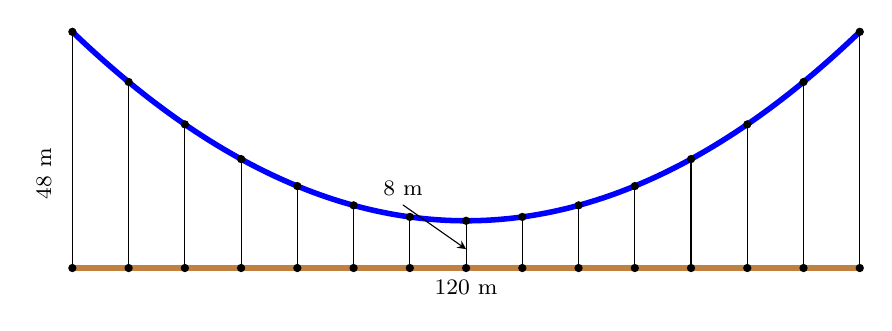
\begin{tikzpicture}[scale=0.8, font=\footnotesize, line join=round, line cap=round, >=stealth]
			\tikzset{thanh-cau/.pic={
					\pgfmathsetmacro\k{5/7};
					\draw[line width=2pt,blue,smooth,samples=100, domain=-5:5] plot (\x,{(12/125)*(\x)^2+0.6});
					\foreach \i in {-7,-6,...,7} \draw ({(\k)*(\i)},0)--({(\k)*(\i)},{(12/125)*((\k)*(\i))^2+0.6});
					\draw[line width=2pt,brown] (-5,0)--(5,0);
					\foreach \i in {-7,-6,...,7} \fill[black] ({(\k)*(\i)},0) circle (1.5pt);
					\foreach \i in {-7,-6,...,7} \fill[black] ({(\k)*(\i)},{(12/125)*((\k)*(\i))^2+0.6}) circle (1.5pt);
			}}
			\path (0,0)pic{thanh-cau};
			\draw (-6.7,1.5) node[rotate=90]{$48$ m};
			\draw (0,-0.3) node{$120$ m};
			\draw[<-] (0,0.3)--(-1,1) node[above]{$8$ m};
		\end{tikzpicture}
	}
	\loigiai{
		\immini{
			Chọn hệ trục tọa độ $Oxy$ như hình vẽ bên dưới.\\
			Gọi phương trình chính tắc của parabol $(P)$ có dạng $y^2=2px$, với $p>0$.\\
			Theo đề parabol $(P)$ đi qua điểm $M(40;60)$ nên $60^2=2p\cdot 40$ hay $p=45$.\\
			Khi đó $(P)\colon y^2=90x$.\\
			Thay tọa độ điểm $N(x_N;20)$ vào phương trình $(P)$, ta được $20^2=90\cdot x_N$.\\
			Suy ra $x_N=\dfrac{40}{9}$.\\
			Vậy chiều dài của thanh cách điểm giữa cầu $20$ m là $\dfrac{40}{9}+8=\dfrac{112}{9}\approx 12{,}44$ (m).
		}{
			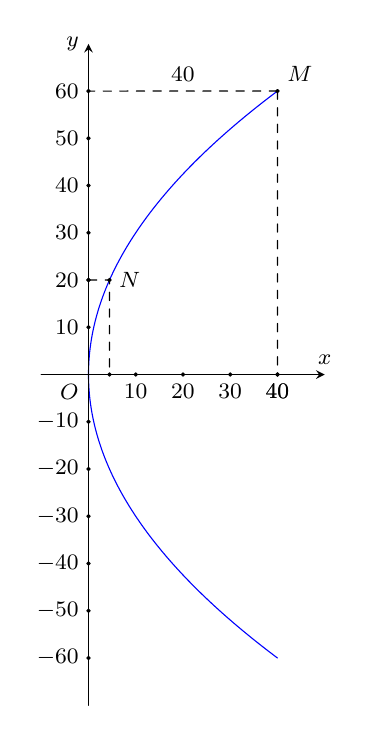
\begin{tikzpicture}[scale=0.6, font=\footnotesize, line join=round, line cap=round, >=stealth]	
				\draw[rotate=-90,blue,smooth,samples=100, domain=-6:6] plot (\x,{(1/9)*(\x)^2});
				\draw[->] (-1,0)--(5,0) node[above]{$x$};
				\draw[->] (0,-7)--(0,7) node[left]{$y$};
				\draw[fill=black] (0,0) node[below left]{$O$};
				\draw [fill=black](4,6) coordinate(M) circle(1pt) node[above right]{$M$};
				\draw [fill=black](0.444,2) coordinate(N) circle(1pt) node[right]{$N$};
				\foreach \i/\m in {1/10,2/20,3/30,4/40} \draw[fill=black] (\i,0) circle(1pt) node[below]{$\m$};
				\foreach \j/\n in {-6/-60,-5/-50,-4/-40,-3/-30,-2/-20,-1/-10,1/10,2/20,3/30,4/40,5/50,6/60} \draw[fill=black] (0,\j) circle(1pt) node[left]{$\n$};
				\draw[dashed] (M)--(0,6) node[above,pos=0.5]{$40$};
				\draw[dashed] (M)--(4,0) coordinate(M_1);
				\draw[dashed] (0,2) coordinate(N_2)--(N)--(0.444,0) coordinate(N_1);
				\draw[fill=black] (M_1) circle(1pt) node[below]{$40$};
				\draw[fill=black] (N_1) circle(1pt);
				\draw[fill=black] (N_2) circle(1pt);
			\end{tikzpicture}
		}
		}
\end{ex}

%Cau20
\begin{ex}%[0H9V5-0]%[Dự án đề cương 3 khối NH 24-25-Dot 2-Nắng Đông]
	\immini{
		Thang leo gợn sóng cho trẻ em trong công viên có hai khung thép cong hình nửa elip cao $100$ cm và khoảng cách giữa hai chân là $240$ cm. Tính khoảng cách thẳng đứng từ một điểm cách chân khung $20$ cm lên đến khung thép. (kết quả làm tròn đến hàng đơn vị)
		\choice
		{\True $55$ cm}
		{$45$ cm}
		{$62$ cm}
		{$47$ cm}
	}{
		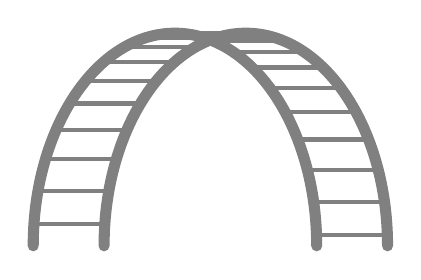
\begin{tikzpicture}[line join = round, line cap = round,>=stealth,x=0.6cm,y=0.6cm]
			\tikzset{Thang-leo/.pic={
					\def\a{3}
					\def\b{1.5*\a}
					\def\d{1.5}
					\draw[gray,line width=4pt](\a,0)arc(0:180:{\a} and {\b});
					\draw[gray,line width=4pt,shift={(\d,0)}](\a,0)arc(0:180:{\a} and {\b});
					\foreach \g in{3,12,...,180}
					\draw[gray,line width=1.5pt](\g: {\a} and {\b})--++(0:\d);
			}}
			\path(0,0)pic{Thang-leo};
		\end{tikzpicture}
	}
	\loigiai{
		Gọi phương trình chính tắc của elip có dạng $$\dfrac{x^2}{a^2}+\dfrac{y^2}{b^2}=1\,,\heva{&a>b>0\\
			&c^2=a^2-b^2.}$$
		Theo đề 
		\begin{itemize}
			\item Khoảng cách giữa hai chân của thang là $240$ cm hay $2a=240$, suy ra $a=120$.
			\item Thang cao $100$ cm hay $b=100$.
		\end{itemize}
		Suy ra phương trình chính tắc của elip là $\dfrac{x^2}{120^2}+\dfrac{y^2}{100^2}=1$.\\
		Thay $x=120-20=100$ vào phương trình elip, ta được $\dfrac{100^2}{120^2}+\dfrac{y^2}{100^2}=1$ hay $y^2=100^2\cdot\left(1-\dfrac{100^2}{120^2}\right)$, suy ra $y \approx 55$.\\
		Vậy khoảng cách thẳng đứng từ một điểm cách chân khung $20$ cm đến khung thép là $55$ cm.
	}
\end{ex}


\Closesolutionfile{ans}

\ind{PHẦN II.} \inden{Câu trắc nghiệm đúng sai. Trong mỗi ý a), b), c), d) ở mỗi câu, học sinh chọn đúng hoặc sai.}\\
\setcounter{ex}{0}
\Opensolutionfile{ans}[ans/2D1-Bai1-DS]%--Đặt tên 2D1-Bai1-DS
%Cau1
\begin{ex}%[0H9H5-1]%[Dự án đề cương 3 khối NH 24-25-Dot 2-Nắng Đông]
	\textit{(Trích đề thi HK2 - Trường THPT Lương Thế Vinh - Hà Nội - Năm học 2023-2024)}\\
	Trong mặt phẳng tọa độ $Oxy$, cho elip $(E)$ có phương trình $\dfrac{x^2}{9}+\dfrac{y^2}{1}=1$.
	\choiceTF
	{\True Các đỉnh nằm trên trục lớn là $A_1(3;0)$ và $A_2(-3;0)$ }
	{Tiêu cự của elip bằng $2$}
	{\True Một tiêu điểm của elip có tọa độ là $F\left(2\sqrt{2};0\right)$}
	{\True Elip có độ dài trục lớn $2a=6$ và độ dài trục bé $2b=2$}
	\loigiai{
		Ta có $(E)\colon \dfrac{x^2}{9}+\dfrac{y^2}{1}=1$. Khi đó
		\begin{itemize}
			\item $a^2=9$, suy ra $a=3$.
			\item $b^2=1$, suy ra $b=1$.
		\end{itemize}
		Và $c^2=a^2-b^2=8$, suy ra $c=2\sqrt{2}$.
		\begin{itemchoice}
			\itemch Các đỉnh nằm trên trục lớn là $A_1(3;0)$ và $A_2(-3;0)$.
			\itemch Tiêu cực của elip bằng $2c=4\sqrt{2}$. 
			\itemch Hai tiêu điểm của elip có tọa độ là $\left(-2\sqrt{2};0\right)$, $\left(2\sqrt{2};0\right)$.
			\itemch Elip có độ dài trục lớn $2a=6$ và độ dài trục bé $2b=2$
		\end{itemchoice}
	}
\end{ex}

%Cau2
\begin{ex}%[0H9H5-0]%[Dự án đề cương 3 khối NH 24-25-Dot 2- Nắng Đông]
\textit{(Trích đề thi HK2 - Trường THPT Chuyên Hùng Vương - Phú Thọ - Năm học 2023-2024)}\\
		Trong mặt phẳng tọa độ $Oxy$, cho đường hypebol $(H)$ có phương trình chính tắc là $\dfrac{x^2}{64}-\dfrac{y^2}{36}=1$.
		\choiceTF
		{Hypebol $(H)$ có tiêu cự bằng $10$}
		{\True Hypebol $(H)$ có một tiêu điểm là $F_2(10;0)$}
		{Điểm $M(0;6)$ thuộc đường hypebol $(H)$}
		{Hiệu các khoảng cách từ một điểm bất kỳ nằm trên đường hypebol $(H)$ đến hai tiêu điểm của $(H)$ có giá trị tuyệt đối bằng $8$}
		\loigiai{Ta có $(H)\colon\dfrac{x^2}{64}-\dfrac{y^2}{36}=1$. Khi đó
			\begin{itemize}
				\item $a^2=64$, suy ra $a=8$.
				\item $b^2=36$, suy ra $b=6$.
			\end{itemize}
			Và $c^2=a^2+b^2=100$, suy ra $c=10$.
			\begin{itemchoice}
				\itemch Tiêu cự của hypebol $(H)$ là $2c=20$.
				\itemch	Hai tiêu điểm của hypebol $(H)$ có toạ độ là $(-10;0)$, $(10;0)$.
				\itemch Thay $M(0;6)$ vào phương trình chính tắc là $\dfrac{x^2}{64}-\dfrac{y^2}{36}=1$ ta được $0-1=1$ (vô lí) nên $M(0;6)$ không thuộc đường hypebol $(H)$.
				\itemch Hiệu các khoảng cách từ một điểm bất kỳ nằm trên đường hypebol $(H)$ đến hai tiêu điểm của $(H)$ có giá trị tuyệt đối bằng $2a=2\cdot 8=16$.
			\end{itemchoice}
		}
	\end{ex}
	
%Cau3
\begin{ex}%[0H9H5-7]%[Dự án đề cương 3 khối NH 24-25-Dot 2-Nắng Đông]
	Trong mặt phẳng toạ độ $Oxy$, cho parabol $(P)$ có phương trình chính tắc là $y^2=24x$.
	\choiceTF
	{\True Tham số tiêu $p=12$}
	{Toạ độ tiêu điểm $F(12;0)$}
	{Phương trình đường chuẩn $x-12=0$}
	{\True Khoảng cách từ tiêu điểm đến đường chuẩn bằng $12$}
	\loigiai{
		\begin{itemchoice}
			\itemch Từ phương trình chính tắc của parabol $(P)$, suy ra $2p=24$ hay $p=12$.
			\itemch Toạ độ tiêu điểm $F(6;0)$.
			\itemch Phương trình đường chuẩn $x=-6$ hay $x+6=0$.
			\itemch Khoảng cách từ tiêu điểm đến đường chuẩn là $p=12$.
		\end{itemchoice}
	}
\end{ex}

%Cau4
\begin{ex}%%[0H9V5-9]%[Dự án đề cương 3 khối NH 24-25-Dot 2-Nắng Đông]
	Trong mặt phẳng toạ độ $Oxy$, cho parabol $(P)\colon y^2=64x$ và đường thẳng $\Delta\colon 4x+3y+46=0$. Gọi $M\left(x_0;y_0\right)$ là điểm trên $(P)$.
	\choiceTF
	{\True $y_0^2=64x_0$}
	{\True Điểm $I(1;-8)\in (P)$}
	{Khoảng cách từ điểm $M$ đến đường thẳng $\Delta$ là $\dfrac{|4x_0+3y_0+46|}{25}$}
	{\True Với $N$ là điểm trên $\Delta$ sao cho độ dài $MN$ ngắn nhất khi đó $x_0+2y_0=-39$}
	\loigiai{
		\begin{itemchoice}
			\itemch Vì $M\left(x_0;y_0\right)$ là điểm trên $(P)\colon y^2=64x$ nên $y_0^2=64x_0$.
			\itemch Thay toạ độ điểm $I$ vào phương trình của parabol $(P)$ ta được $(-8)^2=64\cdot 1$ (đúng) nên $I(1;-8)\in (P)$.
			\itemch Ta có $\mathrm{\,d}\left(M,\Delta\right)=\dfrac{|4x_0+3y_0+46|}{\sqrt{25}}=\dfrac{|4x_0+3y_0+46|}{5}$.
			\itemch Độ dài $MN$ ngắn nhất khi và chỉ khi $\mathrm{\,d}\left(M,\Delta\right)$ nhỏ nhất.\\
			Mà $\mathrm{\,d}\left(M,\Delta\right)=\dfrac{|4x_0+3y_0+46|}{5}=\dfrac{\Big|\dfrac{y_0^2}{16}+3y_0+46\Big|}{5}=\dfrac{1}{5}\left[\left(\dfrac{y_0}{4}+6\right)^2+10\right]\geq \dfrac{1}{5}\cdot 10=2$.\\
			Dấu \lq\lq$=$\rq\rq xảy khi khi và chỉ khi $\dfrac{y_0}{4}+6=0$ hay $y_0=-24$, suy ra $x_0=9$.\\
			Vậy $MN$ ngắn nhất khi $M(9;-24)$ hay $x_0+2y_0=-39$. 
		\end{itemchoice}
	}
\end{ex}
%Cau5
\begin{ex}%[0H9V5-3]%[Dự án đề cương 3 khối NH 24-25-Dot 2-Nắng Đông]
	Trong mặt phẳng tọa độ $Oxy$, cho elip $(E)$ có phương trình $9x^2+25y^2=225$ có hai tiêu điểm $F_1$ và $F_2$.
	\choiceTF
	{\True Hai tiêu điểm của $(E)$ có toạ độ là $(-4;0)$ và $(4;0)$}
	{\True Tỉ số giữa độ dài trục bé và tiêu cự bằng $\dfrac{3}{4}$}
	{\True Với $I$ là điểm trên $(E)$ và $x_I=\dfrac{25}{12}$ thì diện tích tam giác $IF_1F_2$ bằng $\sqrt{119}$ (đvdt)}
	{Có đúng bốn điểm nằm trên $(E)$ và cùng nhìn hai tiêu điểm $F_1$, $F_2$ dưới một góc vuông, khi đó bốn điểm đó tạo thành hình chữ nhật có diện tích lớn hơn $30$}
	\loigiai{
		
		\begin{itemchoice}
			\itemch Ta có $(E)\colon 9x^2+25y^2=225$ hay $\dfrac{x^2}{25}+\dfrac{y^2}{9}=1$. Khi đó
			\begin{itemize}
				\item $a^2=25$, suy ra $a=5$.
				\item $b^2=9$, suy ra $b=3$.
			\end{itemize}
			Và $c^2=a^2-b^2=16$, suy ra $c=4$ hay hai tiêu điểm của $(E)$ có toạ độ là $(-4;0)$ và $(4;0)$.
			\itemch Ta có $\dfrac{2b}{2c}=\dfrac{6}{8}=\dfrac{3}{4}$.
			\itemch Ta có $9x_I^2+25y_I^2=225$ suy ra $25y_I^2=225-9\cdot \left(\dfrac{25}{12}\right)^2$ hay $y_I^2=\dfrac{119}{16}$.\\
			Suy ra $y_I=\pm \dfrac{\sqrt{119}}{4}$.\\
			Khi đó $S_{\Delta{IF_1F_2}}=\dfrac{1}{2}\mathrm{\,d}(I,Ox)\cdot F_1F_2=\dfrac{1}{2}|y_I|\cdot 2c=\sqrt{119}$.
			\itemch Gọi $M(x_0;y_0)$ là điểm trên $(E)$ và $M$ nhìn hai tiêu điểm $F_1$, $F_2$ dưới một góc vuông. Khi đó
			\begin{itemize}
				\item $M\in (E)$ nên $9x_0^2+25y_0^2=225$. \,\hfill (1)
				\item $M$ thuộc đường tròn tâm $O$, đường kính $F_1F_2=8$ nên $x_0^2+y_0^2=16$ \,\hfill (2)
			\end{itemize} 
			Từ (1) và (2) ta có hệ phương trình $\heva{&9x_0^2+25y_0^2=225\\&x_0^2+y_0^2=16}$,
			suy ra $\heva{&x_0^2=\dfrac{175}{16}\\&y_0^2=\dfrac{81}{16}}$ hay $\heva{&x_0=\pm \dfrac{5\sqrt{7}}{4}\\&y_0=\pm\dfrac{9}{4}.}$\\
			Bốn điểm trên $(E)$ nhìn hai tiêu điểm $F_1$, $F_2$ dưới một góc vuông có toạ độ là $\left(\dfrac{5\sqrt{7}}{4};\dfrac{9}{4}\right)$, $\left(\dfrac{5\sqrt{7}}{4};-\dfrac{9}{4}\right)$, $\left(\dfrac{-5\sqrt{7}}{4};-\dfrac{9}{4}\right)$, $\left(\dfrac{-5\sqrt{7}}{4};\dfrac{9}{4}\right)$.\\
			Bốn điểm trên tạo thành hình chữ nhật có diện tích là $2\cdot\dfrac{5\sqrt{7}}{4}\cdot 2\cdot\dfrac{9}{4} \approx 29{,}76$ (đvdt).
		\end{itemchoice}
	}
\end{ex} 
\Closesolutionfile{ans}


\ind{PHẦN III.} \inden{Câu trắc nghiệm trả lời ngắn.}\\
\setcounter{ex}{0}
\Opensolutionfile{ans}[ans/2D1-Bai1-TLN]%--Đặt tên 2D1-Bai1-DS

%Cau1
\begin{ex}%[0H9N5-1]%[Dự án đề cương 3 khối NH 24-25-Dot 2- Nắng Đông]
	\textit{(Trích đề thi HK2 - Trường THPT Chuyên Hùng Vương - Phú Thọ - Năm học 2023-2024)}\\
		Trong mặt phẳng $Oxy$, cho đường elip $(E)$ có phương trình  $\dfrac{x^2}{36}+\dfrac{y^2}{9}=1$. Tổng khoảng cách từ mỗi điểm trên elip tới hai tiêu điểm bằng bao nhiêu?
		\shortans[oly]{12}
		\loigiai{
			Ta có phương trình của chính tắc elip $(E)$ là $\dfrac{x^2}{36}+\dfrac{y^2}{9}=1$.\\
			Suy ra $a^2=36$ hay $a=6$.\\
			Khi đó tổng khoảng cách từ mỗi điểm trên elip tới hai tiêu điểm là $2a=12$.
		}
	\end{ex}
	
%cau2
\begin{ex}%%[0H9H5-4]%[Dự án đề cương 3 khối NH 24-25-Dot 2-Nắng Đông]
	Trong mặt phẳng toạ độ $Oxy$, cho hypebol $(H)$ có độ dài trục thực bằng $2$ và đi qua điểm $M\left(\sqrt{2};-2\right)$. Khi đó tiêu cự của $(H)$ bằng $m$, tính giá trị của $m^4+2\,025$.
	\shortans[oly]{2425}
	\loigiai{
		Gọi phương trình chính tắc của hypebol có dạng $$\dfrac{x^2}{a^2}-\dfrac{y^2}{b^2}=1\,,\heva{&a,b>0\\
			&c^2=a^2+b^2.}$$
		Theo đề 
		\begin{itemize}
			\item Độ dài trục thực bằng $2$ nên $2a=2$, suy ra $a=1$.
			\item $(H)$ đi qua điểm $M\left(\sqrt{2};-2\right)$ suy ra $\dfrac{2}{a^2}-\dfrac{4}{b^2}=1$ hay $\dfrac{2}{1}-\dfrac{4}{b^2}=1$, từ đó ta được $b^2=4$.
		\end{itemize}
		Và $c^2=a^2+b^2=5$, suy ra $c=\sqrt{5}$ hay tiêu cự của $(H)$ là $2c=2\sqrt{5}$.\\
		Vậy $m=2\sqrt{5}$ hay $m^4+2\,025=400+2\,025=2\,425$.
	}
\end{ex}
%Cau3
\begin{ex}%[0H9V5-0]%[Dự án đề cương 3 khối NH 24-25-Dot 2-Nắng Đông]
	\immini{Một chiếc đèn có mặt cắt ngang là hình parabol như hình bên. Hình parabol có chiều rộng giữa hai mép vành là $AB=40$cm và chiều sâu $h=30$cm ($h$ bằng khoảng cách từ $O$ đến $AB$). Bóng đèn nằm ở tiêu điểm $S$. Khoảng cách từ bóng đèn đến đường chuẩn của parabol là bao nhiêu cm? (kết quả làm tròn đến hàng phần chục)}
	{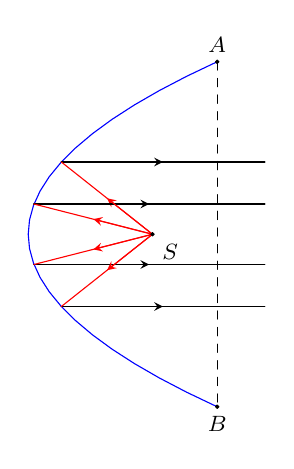
\begin{tikzpicture}[scale=0.6, font=\footnotesize, line join=round, line cap=round, >=stealth]
			\draw[domain=-3.65:3.65, blue,] plot({3/10*(\x)^2},\x);
			\coordinate (A) at (4,3.65); 
			\coordinate (B) at (4,-3.65); 
			\coordinate (O) at (0,0); 
			\coordinate (C) at (0.12,0.64); 
			\coordinate (C') at (0.12,-0.64); 
			\coordinate (D) at (0.7,1.53); 
			\coordinate (D') at (0.7,-1.53); 
			\coordinate (F) at (5.01,1.53); 
			\coordinate (F') at (5.01,-1.53); 
			\coordinate (G) at (5.01,0.64); 
			\coordinate (G') at (5.01,-0.64); 
			\coordinate (E) at (2.63,0); 
			\coordinate (H1) at (1.67,0.76); 
			\coordinate (H2) at (1.67,-0.76); 
			\coordinate (H3) at (1.38,0.32); 
			\coordinate (H4) at (1.38,-0.32); 
			\coordinate (K1) at (2.85,1.53); 
			\coordinate (K2) at (2.85,-1.53); 
			\coordinate (K3) at (2.56,0.64); 
			\coordinate (K4) at (2.56,-0.64); 
			\draw (F)--(D) (G)--(C) (F')--(D') (G')--(C') ;
			\draw[dashed] (A)--(B);
			\draw[red,->] (E)--(H1); 
			\draw[->] (D)--(K1) ;
			\draw[red,->] (E)--(H3); 
			\draw[->] (C)--(K3) ;
			\draw[red,->] (E)--(H4); 
			\draw[->] (C')--(K4) ;
			\draw[red,->] (E)--(H2); 
			\draw[->] (D')--(K2) ;
			\draw[red] (E)--(C) (E)--(D) (E)--(C') (E)--(D');
			\draw[fill=black] (A) circle (1pt) node [above] {$A$};
			\draw[fill=black] (B) circle (1pt) node [below] {$B$};
			\draw[fill=black] (E) circle (1pt) node [below right] {$S$};
	\end{tikzpicture}}
	\shortans[oly]{6,7}
	\loigiai{
		Chọn hệ trục toạ độ $Oxy$ như hình vẽ bên dưới.
		\begin{center}
			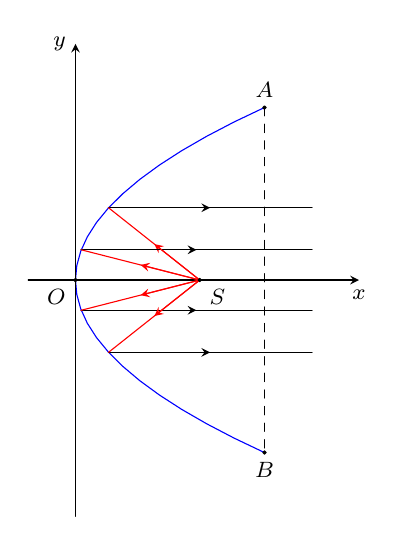
\begin{tikzpicture}[scale=0.6, font=\footnotesize, line join=round, line cap=round, >=stealth]
				\draw[domain=-3.65:3.65, blue,] plot({3/10*(\x)^2},\x);
				%\draw[gray!10] (-1,-1) grid (5,5);
				\draw[->] (-1,0)--(6,0) node[below]{$x$};
				\draw[->] (0,-5)--(0,5) node[left]{$y$};
				\coordinate (A) at (4,3.65); 
				\coordinate (B) at (4,-3.65); 
				\coordinate (O) at (0,0); 
				\coordinate (C) at (0.12,0.64); 
				\coordinate (C') at (0.12,-0.64); 
				\coordinate (D) at (0.7,1.53); 
				\coordinate (D') at (0.7,-1.53); 
				\coordinate (F) at (5.01,1.53); 
				\coordinate (F') at (5.01,-1.53); 
				\coordinate (G) at (5.01,0.64); 
				\coordinate (G') at (5.01,-0.64); 
				\coordinate (E) at (2.63,0); 
				\coordinate (H1) at (1.67,0.76); 
				\coordinate (H2) at (1.67,-0.76); 
				\coordinate (H3) at (1.38,0.32); 
				\coordinate (H4) at (1.38,-0.32); 
				\coordinate (K1) at (2.85,1.53); 
				\coordinate (K2) at (2.85,-1.53); 
				\coordinate (K3) at (2.56,0.64); 
				\coordinate (K4) at (2.56,-0.64); 
				\draw (F)--(D) (G)--(C) (F')--(D') (G')--(C') ;
				\draw[dashed] (A)--(B);
				\draw[red,->] (E)--(H1); 
				\draw[->] (D)--(K1) ;
				\draw[red,->] (E)--(H3); 
				\draw[->] (C)--(K3) ;
				\draw[red,->] (E)--(H4); 
				\draw[->] (C')--(K4) ;
				\draw[red,->] (E)--(H2); 
				\draw[->] (D')--(K2) ;
				\draw[red] (E)--(C) (E)--(D) (E)--(C') (E)--(D');
				\draw[fill=black] (A) circle (1pt) node [above] {$A$};
				\draw[fill=black] (B) circle (1pt) node [below] {$B$};
				\draw[fill=black] (E) circle (1pt) node [below right] {$S$};
				\draw[fill=black] (O) circle (1pt) node [below left] {$O$};
			\end{tikzpicture}
		\end{center}
		Gọi phương trình chính tắc của parabol có dạng $y^2=2px$, với $p>0$.\\
		Theo đề parabol đi qua điểm $A(30;20)$ nên ta có phương trình $20^2=2p\cdot 30$ suy ra $p=\dfrac{20}{3}$.\\
		Khi đó phương trình đường chuẩn của parabol đó là $x=-\dfrac{10}{3}$.\\
		Vậy khoảng cách từ bóng đèn đến đường chuẩn của parabol là $p=\dfrac{20}{3}\approx 6{,}7$ cm.
	}
\end{ex}
%Cau4
\begin{ex}%[0H9V5-0]%[Dự án đề cương 3 khối NH 24-25-Dot 2-Nắng Đông]
	Mặt Trăng chuyển động quanh Trái Đất theo quỹ đạo là một đường elip với tâm Trái Đất là một tiêu điểm. Độ dài trục lớn, trục nhỏ của quỹ đạo lần lượt là $768\,800$ km và $767\,640$ km. Khoảng cách nhỏ nhất từ tâm Trái Đất đến Mặt Trăng là bao nhiêu nghìn km? (kết quả làm tròn đến hàng đơn vị)
	\shortans[oly]{356}
	\loigiai{
		Gọi phương trình chính tắc của elip có dạng $$\dfrac{x^2}{a^2}+\dfrac{y^2}{b^2}=1\,,\heva{&a>b>0\\
			&c^2=a^2-b^2.}$$
		Theo đề 
		\begin{itemize}
			\item $2a=768\,800$, suy ra $a=384\,400$.
			\item $2b=767\,640$, suy ra $b=383\,320$.
		\end{itemize}
		Từ đó suy ra $c=\sqrt{a^2-b^2}=\sqrt{384\,400^2-383\,320^2}$.\\
		Khoảng cách nhỏ nhất từ tâm Trái Đất đến Mặt Trăng là
		$$a-c=384\,400-\sqrt{384\,400^2-383\,320^2}\approx 355\,605\,\text{ (km)}.$$
		Vậy khoảng cách nhỏ nhất từ tâm Trái Đất đến Mặt Trăng là $356$ nghìn km.
	}
\end{ex}
%Cau5
\begin{ex}%[0H9V5-0]%[Dự án đề cương 3 khối NH 24-25-Dot 2-Nắng Đông]
	\immini{
		Mặt cắt của một tháp làm nguội của một nhà máy là một hypebol có độ dài trục ảo bằng $80$. Khoảng cách từ nóc tháp đến tâm đối xứng bằng nửa khoảng cách từ tâm đối xứng đến đáy (hình vẽ). Tính chiều cao của tháp, biết bán kính đường tròn nóc và bán kính đường tròn đáy tháp lần lượt là $27 \sqrt{2}$ mét và $27 \sqrt{5}$ mét.
	}
	{
		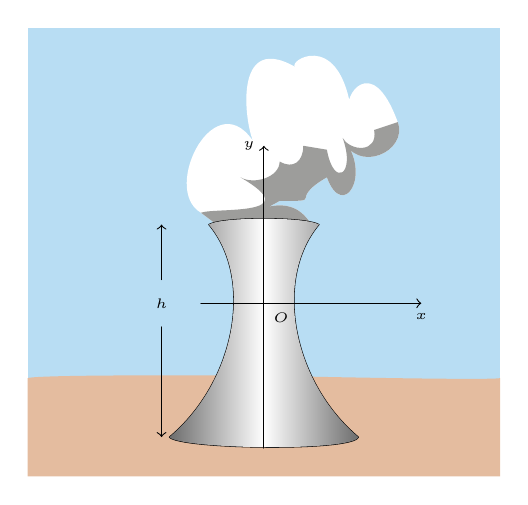
\begin{tikzpicture}[line join=round, line cap=round,scale=1,transform shape]
			\definecolor{lightcornflowerblue}{rgb}{0.6, 0.81, 0.93}
			\definecolor{tumbleweed}{rgb}{0.87, 0.67, 0.53}
			\definecolor{dimgray}{rgb}{0.41, 0.41, 0.41}
			\definecolor{battleshipgrey}{rgb}{0.52, 0.52, 0.51}
			\def\xmin{-.8} \def\xmax{2}
			\def\ymin{-1.84} \def\ymax{2} 
			
			\fill[lightcornflowerblue!70] (-3,-2) rectangle (3,3.5);
			\tikzset{thap/.pic={
					\def\C{ %Cát
						(-3,-.65)
						..controls +(15:.2) and +(120:0) .. (0,-.62)
						..controls +(-60:0) and +(-160:0.1) .. (3,-.65)--(3,-1.9)--(-3,-1.9)--cycle
						;}
					%\draw \C;
					\fill[tumbleweed!80] \C;
					
					\def\D{ 
						(-.7,1.3)
						..controls +(-50:.9) and +(40:1.1) .. (-1.2,-1.4)
						..controls +(-50:0.2) and +(-110:0.2) .. (1.2,-1.4)
						..controls +(140:1.1) and +(-130:.9) .. (.7,1.3)
						..controls +(150:0.2) and +(30:0.2) .. (-.7,1.3)
						;}
					\draw \D;
					\fill[left color=dimgray!97,right color=dimgray!97, middle color=white] \D;
					\draw[->] (-1.3,0.6)--(-1.3,1.3);
					\draw[<-] (-1.3,-1.4)--(-1.3,0);
			}}
			
			\fill[white] (-.8,1.15)
			..controls +(150:.6) and +(120:1) .. (-.1,2)
			..controls +(150:.13) and +(150:1) .. (.4,3)
			..controls +(150:.13) and +(100:1) .. (1.1,2.5)
			..controls +(150:.13) and +(110:1) .. (1.7,2.3)
			..controls +(-70:.4) and +(-70:.5) .. (1,2.1)
			..controls +(-50:.6) and +(-70:.6) .. (.8,1.6)
			..controls +(-150:.6) and +(0:.6) .. (.2,1.3)
			..controls +(-150:.6) and +(120:.6) .. (.6,1)--(-.6,1)--cycle;
			
			\fill[battleshipgrey!80] (-.6,1)--(-.8,1.15)
			..controls +(20:.2) and +(-30:1) .. (-.3,1.6)
			..controls +(-30:.2) and +(-90:.2) .. (.2,1.8)
			..controls +(-30:.2) and +(-90:.2) .. (.5,2)--(.8,1.95)
			..controls +(-80:.5) and +(-70:.5) .. (1,2.1)
			..controls +(-60:.2) and +(-80:.3) .. (1.4,2.2)--(1.7,2.3)
			..controls +(-70:.4) and +(-70:.5) .. (1,2.1)
			..controls +(-50:.6) and +(-70:.6) .. (.8,1.6)
			..controls +(-150:.6) and +(0:.6) .. (.2,1.3)
			..controls +(-150:.6) and +(120:.6) .. (.6,1)--cycle
			;
			%%%%%%%%%%%%%%%%%%
			
			\path(0,-0.3)pic[scale=1]{thap};
			\draw[->] (\xmin,0)--(\xmax,0) node [below]{\tiny $x$};
			\draw[->] (0,\ymin)--(0,\ymax) node [left]{\tiny $y$};
			\node at (0,0) [below right]{\tiny $O$};	
			\node at (-1.3,0) {\tiny $h$};	
		\end{tikzpicture}
	}
	\shortans[oly]{120}
	\loigiai{Gọi phương trình chính tắc của hypebol $(H)$ có dạng $$\dfrac{x^2}{a^2}-\dfrac{y^2}{b^2}=1\,,\heva{&a,b>0\\
			&c^2=a^2+b^2.}$$
		Theo đề 
		\begin{itemize}
			\item Độ dài trục ảo $2b=80$ nên $b=40$.
			\item $(H)$ đi qua điểm $M(27\sqrt{2};y)$ ở đỉnh tháp và điểm $N(27\sqrt{5};2y)$ ở đáy tháp nên ta có hệ phương trình
			$\heva{&\dfrac{\left(27 \sqrt{2}\right)^2}{a^2}-\dfrac{y^2}{40^2}=1 \\
				&\dfrac{\left(27 \sqrt{5}\right)^2}{a^2}-\dfrac{4 y^2}{40^2}=1.}$
		\end{itemize}
		Giải hệ phương trình trên, ta được $\heva{&\dfrac{1}{a^2}=\dfrac{1}{729} \\
			&y^2=1600}$	hay $\heva{&a=27 \\&y=40.}$\\
		Do đó $h=y+2y=120$.\\
		Vậy chiều cao của tháp là $120$ mét.
	}
\end{ex}

\Closesolutionfile{ans}


\ind{PHẦN IV.} \inden{Tự luận.}\\
\setcounter{ex}{0}
%Cau1

\begin{ex}%%[0H9H5-1]%[Dự án đề cương 3 khối NH 24-25-Dot 2-Nắng Đông]
	Trong mặt phẳng toạ độ $Oxy$, cho phương trình chính tắc của elip $(E)\colon \dfrac{x^2}{16}+\dfrac{y^2}{9}=1$. Hãy xác định toạ độ các đỉnh; độ dài trục lớn, trục bé; tiêu điểm và tiêu cự của elip $(E)$.
	\loigiai{
		Từ phương trình chính tắc của elip $(E)\colon \dfrac{x^2}{16}+\dfrac{y^2}{9}=1$, ta có
		\begin{itemize}
			\item $a^2=16$, suy ra $a=4$.
			\item $b^2=9$, suy ra $b=3$.
			\item $c^2=a^2-b^2=7$, suy ra $c=\sqrt{7}$.
		\end{itemize}
		Khi đó
		\begin{itemize}
			\item Toạ độ các đỉnh $A_1(-4;0)$, $A_2(4;0)$, $B_1(0;-3)$ và $B_2(0;3)$.
			\item Độ dài trục lớn $2a=8$; độ dài trục bé $2b=6$.
			\item Toạ độ tiêu điểm $F_1\left(-\sqrt{7};0\right)$, $F_2\left(\sqrt{7};0\right)$.
			\item Tiêu cự $2c=2\sqrt{7}$.
		\end{itemize}
	}
\end{ex}

%Cau2
\begin{ex}%%[0H9H5-4]%[Dự án đề cương 3 khối NH 24-25-Dot 2-Nắng Đông]
	Trong mặt phẳng toạ độ $Oxy$, cho phương trình chính tắc của hypebol $(H)\colon \dfrac{x^2}{36}-\dfrac{y^2}{64}=1$. Hãy xác định toạ độ các đỉnh; độ dài trục thực, trục ảo; tiêu điểm và tiêu cự của hypebol $(H)$.
	\loigiai{
		Từ phương trình chính tắc của hypebol $(H)\colon \dfrac{x^2}{36}-\dfrac{y^2}{64}=1$, ta có
		\begin{itemize}
			\item $a^2=36$, suy ra $a=6$.
			\item $b^2=64$, suy ra $b=8$.
			\item $c^2=a^2+b^2=100$, suy ra $c=10$.
		\end{itemize}
		Khi đó
		\begin{itemize}
			\item Toạ độ các đỉnh $A_1(-6;0)$, $A_2(6;0)$.
			\item Độ dài trục thực $2a=12$; độ dài trục ảo $2b=26$.
			\item Toạ độ tiêu điểm $F_1\left(-10;0\right)$, $F_2\left(10;0\right)$.
			\item Tiêu cự $2c=20$.
		\end{itemize}
	}
\end{ex}
%Cau3
\begin{ex}%%[0H9H5-7]%[Dự án đề cương 3 khối NH 24-25-Dot 2-Nắng Đông]
	Trong mặt phẳng toạ độ $Oxy$, cho parabol $(P)$ có phương trình $y^2=24x$.
	\begin{enumerate}
		\item Hãy xác định toạ độ tiêu điểm $F$ của $(P)$.
		\item Tìm phương trình đường chuẩn $\Delta$ của $(P)$.
	\end{enumerate}
	\loigiai{
		Từ phương trình của parabol $(P)\colon y^2=26x$ suy ra tham số tiêu $p=13$.
		Khi đó
		\begin{enumerate}
			\item Toạ độ tiêu điểm $F\left(\dfrac{13}{2};0\right)$.
			\item Phương trình đường chuẩn $\Delta\colon x=-\dfrac{13}{2}$.
		\end{enumerate}
	}
\end{ex}
%Cau4
\begin{ex}%[0H9N5-2]%[Dự án đề cương 3 khối NH 24-25-Dot 2- Nắng Đông]
	Trong mặt phẳng tọa độ $Oxy$, viết phương trình chính tắc của elip $(E)$ có độ dài trục lớn là $8$, tiêu cự bằng $2\sqrt{5}$.
	\loigiai{
		Gọi phương trình chính tắc của elip $(E)$ có dạng $$\dfrac{x^2}{a^2}+\dfrac{y^2}{b^2}=1\,,\heva{&a>b>0\\
			&c^2=a^2-b^2.}$$
		Theo đề 
		\begin{itemize}
			\item $2a=8$, suy ra $a=4$.
			\item $2c=2\sqrt{5}$, suy ra $c=\sqrt{5}$.
		\end{itemize}
		Và $b^2=a^2-c^2=16-5=11$, suy ra $b=\sqrt{11}$.\\
		Vậy phương trình chính tắc của elip $(E)$ là $\dfrac{x^2}{16}+\dfrac{y^2}{11}=1$. 
	}
\end{ex}

%cau5
\begin{ex}%[0H9N5-4]%[Dự án đề cương 3 khối NH 24-25-Dot 2-Nắng Đông]
	\textit{(Trích đề thi HK2 - Trường THPT Nguyễn Thị Minh Khai - TP.HCM - Năm học 2023-2024)}\\
		Trong mặt phẳng tọa độ $Oxy$, cho hypebol $(H)$ có độ dài trục thực bằng $12$ và độ dài tiêu cự bằng $20$. Viết phương trình chính tắc của hypebol $(H)$.
		\loigiai{Gọi phương trình chính tắc của hypebol $(H)$ có dạng $$\dfrac{x^2}{a^2}-\dfrac{y^2}{b^2}=1\,,\heva{&a,b>0\\
				&c^2=a^2+b^2.}$$
			Theo đề 
			\begin{itemize}
				\item $2a=12$, suy ra $a=6$.
				\item $2c=20$, suy ra $c=10$.
			\end{itemize}
			Và $b^2=c^2-a^2=10^2-6^2=64$, suy ra $b=8$.\\
			Vậy phương trình chính tắc của hypebol $(H)$ là $\dfrac{x^2}{36}-\dfrac{y^2}{64}=1$. 
		} 
\end{ex}

%Cau6
\begin{ex}%%[0H9H5-9]%[Dự án đề cương 3 khối NH 24-25-Dot 2-Nắng Đông]
	Trong mặt phẳng toạ độ $Oxy$, cho parabol $(P)\colon y^2=25x$. Gọi $M$ là điểm trên $(P)$ biết $M$ có tung độ bằng $-15$. Tính độ dài $OM$.
	\loigiai{
		Gọi $M\left(x_M;y_M\right)$ là điểm trên parabol $(P)$, suy ra $y_M^2=25x_M$.\\
		Theo đề: $y_M=-15$ nên $225=25x_M$, suy ra $x_M=9$.\\
		Vậy $M\left(9;-15\right)$, suy ra $OM=\sqrt{81+225}=3\sqrt{34}$ (đvđd).
	}
\end{ex}


%Cau7
\begin{ex}%[0H9H5-1]%[0H9H5-3]%[Dự án đề cương 3 khối NH 24-25-Dot 2-Nắng Đông]
	\textit{(Trích đề thi HK2 - Trường THPT Gia Định - TP.HCM - Năm học 2023-2024)}\\
		Trong mặt phẳng toạ độ $Oxy$, cho elip $(E)\colon 7x^2+16y^2=112$.
		\begin{enumerate}
			\item Tìm tọa độ các tiêu điểm, tọa độ các đỉnh, tiêu cự và độ dài các trục của $(E)$.
			\item Gọi $M$, $N$ là các điểm trên $(E)$ sao cho $NF_1+MF_2=7$. Tính giá trị $MF_1+NF_2$ với $F_1$, $F_2$ là hai tiêu điểm của $(E)$.
		\end{enumerate}
		\loigiai{
			Ta có $(E)\colon 7x^2+16y^2=112$ hay $\dfrac{x^2}{16}+\dfrac{y^2}{7}=1$. Khi đó
			\begin{itemize}
				\item $a^2=16$, suy ra $a=4$.
				\item $b^2=7$, suy ra $b=\sqrt{7}$.
			\end{itemize}
			Và $c^2=a^2-b^2=9$, suy ra $c=3$.
			\begin{enumerate}
				\item Tọa độ các đỉnh $A_1(-4;0)$, $A_2(4;0)$, $B_1(0;-\sqrt{7})$, $B_2(0;\sqrt{7})$.\\
				Độ dài trục lớn $2a=8$, độ dài trục bé $2b=2\sqrt{7}$.\\
				Tọa độ các tiêu điểm $F_1(-3;0)$, $F_2(3;0)$.\\
				Tiêu cự $2c=6$.
				\item Ta có $M$, $N$ là các điểm trên $(E)$ nên $MF_1+MF_2=8$ và $NF_1+NF_2=8$.\\
				Suy ra $MF_1+MF_2 + NF_1+NF_2=16$.\\
				Mà $NF_1+MF_2=7$ nên $MF_1+NF_2=16-(NF_1+MF_2)=16-7=9$.
			\end{enumerate}
		}
\end{ex}
%Cau8
\begin{ex}%[0H9V5-0]%[Dự án đề cương 3 khối NH 24-25-Dot 2-Nắng Đông]
	\immini{Một kĩ sư thiết kế đường hầm một chiều có mặt cắt là một nửa hình elip, chiều rộng của hầm là $12$ m, khoảng cách từ điểm cao nhất của elip so với mặt đường là $3$ m. Người kĩ sư này muốn đưa ra cảnh báo cho các loại xe có thể đi qua hầm. Biết rằng những loại xe tải có chiều cao $2{,}8$ m thì có chiều rộng không quá $3$ m. Hỏi chiếc xe tải có chiều cao $2{,}8$ m có thể đi qua hầm được không?
	}
	{\begin{tikzpicture}[scale=0.7, font=\footnotesize, line join=round, line cap=round, >=stealth]
			\path
			(-4,0) coordinate (A)
			(-4,2.5) coordinate (B)
			(4,2.5) coordinate (C)
			(4,0) coordinate (D)
			($(A)!0.75!(D)$) coordinate (E)
			($(A)!0.25!(D)$) coordinate (F)
			;
			% miền tường gạch
			\fill[brown!50] (A)--(B)--(C)--(D)--(A);
			\pattern[pattern color=black!70,pattern=bricks] (A)--(B)--(C)--(D)--(A);
			%elip
			\fill [color=black!60](E) arc(0:180:2 and 1.6)--($(F)+(-0.3,0)$)arc(180:0:2.3 and 1.9)--cycle;
			\fill [bottom color=black!70,top color=gray] (B)--(C)--($(C)+(0,0.3)$)-|(B);
			\fill [color=white](E) arc(0:180:2 and 1.6)--cycle;
			\draw [color=black](E) arc(0:180:2 and 1.6);
			\draw [<->]($(F)+(0,-0.8)$)--($(E)+(0,-0.8)$)node[fill=white,midway]{$12$ m};
			\draw [<->]($(A)+(-0.5,0)$)--++(0,1.6)node[fill=white,midway]{$3$ m};
			\draw[dashed] ($(0,0)+(0,1.6)$)--($(A)+(-0.7,1.6)$);
			\draw[dashed] (F)--($(F)+(0,-0.8)$) (E)--($(E)+(0,-0.8)$);
	\end{tikzpicture}}
	\loigiai{
		Chọn hệ trục tọa độ $Oxy$ có tâm $O$ chính giữa đường, trục $Oy$ hướng lên trên như hình vẽ bên dưới. 
		\begin{center}
			\begin{tikzpicture}[xscale=1.3, font=\footnotesize, line join=round, line cap=round, >=stealth]
				\path
				(-4,0) coordinate (A)
				(-4,2.5) coordinate (B)
				(4,2.5) coordinate (C)
				(4,0) coordinate (D)
				($(A)!0.75!(D)$) coordinate (E)
				($(A)!0.25!(D)$) coordinate (F)
				;
				% miền tường gạch
				\fill[brown!50] (A)--(B)--(C)--(D)--(A);
				\pattern[pattern color=black!70,pattern=bricks] (A)--(B)--(C)--(D)--(A);
				%elip
				\fill [color=black!60](E) arc(0:180:2 and 1.6)--($(F)+(-0.3,0)$)arc(180:0:2.3 and 1.9)--cycle;
				\fill [bottom color=black!70,top color=gray] (B)--(C)--($(C)+(0,0.3)$)-|(B);
				\fill [color=white](E) arc(0:180:2 and 1.6)--cycle;
				\draw [color=black](E) arc(0:180:2 and 1.6);
				%hệ trục
				\draw[->] ($(A)+(-0.7,0)$)--($(D)+(0.7,0)$) node[below]{$x$};
				\draw[->] (0,0)--(0,3.5) node[left]{$y$};
				\draw[fill=black](0,0) circle(1pt) node[below]{$O$};
				\draw [<->]($(F)+(0,-0.8)$)--($(E)+(0,-0.8)$)node[fill=white,midway]{$12$ m};
				\draw [<->]($(A)+(-0.5,0)$)--++(0,1.6)node[fill=white,midway]{$3$ m};
				\draw[dashed] ($(0,0)+(0,1.6)$)--($(A)+(-0.7,1.6)$);
				\draw[dashed] (F)--($(F)+(0,-0.8)$) (E)--($(E)+(0,-0.8)$);
				\draw[dashed] (0.5,0)node[below]{$1{,}5$}--(0.5,1.5)node[below left]{$N$};
			\end{tikzpicture}
		\end{center}
		Gọi phương trình chính tắc của elip có dạng là $$\dfrac{x^2}{a^2}+\dfrac{y^2}{b^2}=1\,,\heva{&a>b>0\\
			&c^2=a^2-b^2.}$$
		Theo đề 
		\begin{itemize}
			\item $2a=12$ suy ra $a=6$.
			\item $b=3$.
		\end{itemize}
		Suy ra phương trình chính tắc của elip $(E)$ là $\dfrac{x^2}{36}+\dfrac{y^2}{9}=1$.\\
		Xét một chiếc xe tải có chiều cao $2{,}8$ m. Khi đó chiều rộng không quá $3$ m. Nên tính từ chính giữa xe ra mỗi bên có chiều rộng không qua $1{,}5$ m. Xe sẽ đi được qua hầm nếu điểm $M(1{,}5;2{,}8)$ nằm bên trong elip.\\
		Gọi $N$ là điểm thuộc nửa elip có hoành độ $x_N=1{,}5$.\\
		Khi đó $\dfrac{1{,}5^2}{36}+\dfrac{y_N^2}{9}=1$, suy ra $y_N^2=\dfrac{135}{36}$ hay $y_N=\dfrac{3\sqrt{15}}{4}\approx 2{,}905>2{,}8$.\\
		Vậy điểm $M(1{,}5;2{,}8)$ nằm bên trong elip nên xe đi được qua hầm. Tuy nhiên, cần khuyến cáo ô tô đi vào chính giữa hầm.
		}
\end{ex}
	
%Cau9
\begin{ex}%%[0H9V5-0]%[Dự án đề cương 3 khối NH 24-25-Dot 2-Nắng Đông]
	Một cái cầu có dây cáp treo hình parabol, cầu dài $100$ m và được nâng đỡ bởi những thanh thẳng đứng treo từ cáp xuống, thanh dài nhất là $30$ m, thanh ngắn nhất là $6$ m (hình bên dưới). Tính chiều dài của thanh cách điểm giữa cầu $18$ m.
	\begin{center}
		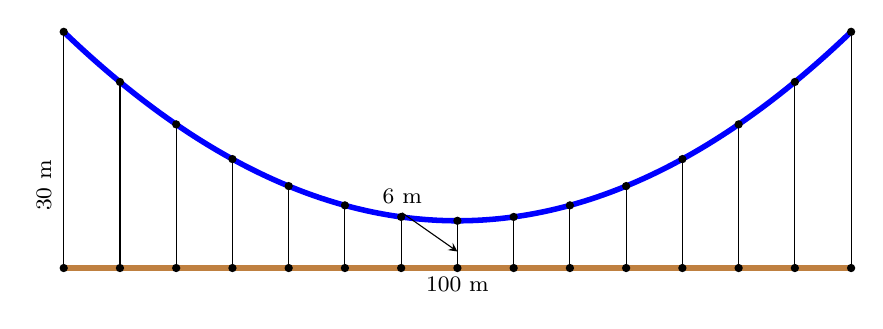
\begin{tikzpicture}[scale=0.7, font=\footnotesize, line join=round, line cap=round, >=stealth]
			\tikzset{thanh-cau/.pic={
					\pgfmathsetmacro\k{5/7};
					\draw[line width=2pt,blue,smooth,samples=100, domain=-5:5] plot (\x,{(12/125)*(\x)^2+0.6});
					\foreach \i in {-7,-6,...,7} \draw ({(\k)*(\i)},0)--({(\k)*(\i)},{(12/125)*((\k)*(\i))^2+0.6});
					\draw[line width=2pt,brown] (-5,0)--(5,0);
					\foreach \i in {-7,-6,...,7} \fill[black] ({(\k)*(\i)},0) circle (1.5pt);
					\foreach \i in {-7,-6,...,7} \fill[black] ({(\k)*(\i)},{(12/125)*((\k)*(\i))^2+0.6}) circle (1.5pt);
			}}
			\path (0,0)pic{thanh-cau};
			\draw (-7.5,1.5) node[rotate=90]{$30$ m};
			\draw (0,-0.3) node{$100$ m};
			\draw[<-] (0,0.3)--(-1,1) node[above]{$6$ m};
		\end{tikzpicture}
	\end{center}
	\loigiai{
		\immini{
			Chọn hệ trục tọa độ $Oxy$ như hình vẽ bên dưới.\\
			Gọi phương trình chính tắc của parabol $(P)$ có dạng $y^2=2px$, với $p>0$.\\
			Theo đề parabol $(P)$ đi qua điểm $M(24;50)$ nên $50^2=2p\cdot 24$ hay $p=\dfrac{625}{12}$.\\
			Khi đó $(P)\colon y^2=\dfrac{625}{6}x$.\\
			Thay tọa độ điểm $N(x_N;18)$ vào phương trình $(P)$, ta được $18^2=\dfrac{625}{6}\cdot x_N$.\\
			Suy ra $x_N=\dfrac{1\,944}{625}=3{,}1104$.\\
			Vậy chiều dài của thanh cách điểm giữa cầu $18$ m là $3{,}1104+6=9{,}1104$ (m).
		}{
			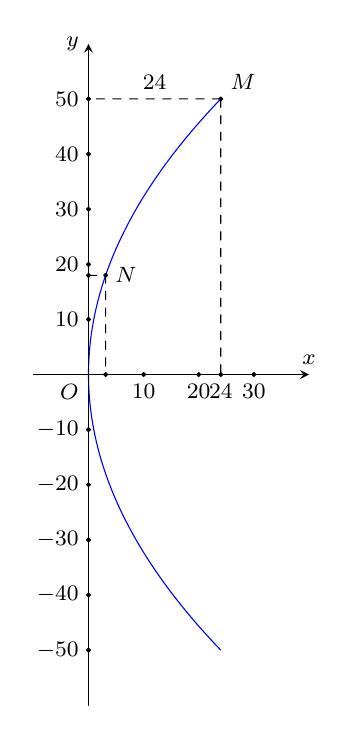
\begin{tikzpicture}[scale=0.7, font=\footnotesize, line join=round, line cap=round, >=stealth]	
				\draw[rotate=-90,blue,smooth,samples=100, domain=-5:5] plot (\x,{(12/125)*(\x)^2});
				\draw[->] (-1,0)--(4,0) node[above]{$x$};
				\draw[->] (0,-6)--(0,6) node[left]{$y$};
				\draw[fill=black] (0,0) node[below left]{$O$};
				\draw [fill=black](2.4,5) coordinate(M) circle(1pt) node[above right]{$M$};
				\draw [fill=black](0.31104,1.8) coordinate(N) circle(1pt) node[right]{$N$};
				\foreach \i/\m in {1/10,2/20,3/30} \draw[fill=black] (\i,0) circle(1pt) node[below]{$\m$};
				\foreach \j/\n in {-5/-50,-4/-40,-3/-30,-2/-20,-1/-10,1/10,2/20,3/30,4/40,5/50} \draw[fill=black] (0,\j) circle(1pt) node[left]{$\n$};
				\draw[dashed] (M)--(0,5) node[above,pos=0.5]{$24$};
				\draw[dashed] (M)--(2.4,0) coordinate(M_1);
				\draw[dashed] (0,1.8) coordinate(N_2)--(N)--(0.31104,0) coordinate(N_1);
				\draw[fill=black] (M_1) circle(1pt) node[below]{$24$};
				\draw[fill=black] (N_1) circle(1pt);
				\draw[fill=black] (N_2) circle(1pt);
			\end{tikzpicture}
		}
	}
\end{ex}
%Cau10
\begin{ex}%[0H9V5-0]%[Dự án đề cương 3 khối NH 24-25-Dot 2-Nắng Đông]
	\textit{(Trích đề thi HK2 - Trường THPT Lê Quý Đôn - TP.HCM - Năm học 2023-2024)}\\
		\immini{
			Một mảnh vườn hình elip như hình vẽ. Biết độ dài các đoạn thẳng $AB = 20$ m;
			$CD = 12$ m, $I$ là trung điểm của $OA$ và các điểm $M$, $N$, $P$, $Q$ đều nằm trên elip và tạo thành một hình chữ nhật. Người ta trồng hoa toàn bộ diện tích hình chữ nhật $MNPQ$. Biết số tiền để trồng hoàn thiện $1$ m$^2$ hoa là $250\,\,000$ đồng. Tổng số tiền để trồng hoa là bao nhiêu triệu đồng? (Kết quả làm tròn đến hàng đơn vị)
		}{
			\begin{tikzpicture}[>=stealth,line join=round,line cap=round,font=\footnotesize,scale=0.7]
				\path
				(0,0) coordinate (O)
				(2.5,0) coordinate (A)
				(-2.5,0) coordinate (B)
				(0,1.8) coordinate (C)
				(0,-1.8) coordinate (D)
				($(O)!0.5!(A)$) coordinate (I)
				(1.25,1.55) coordinate (M)
				(1.25,-1.55) coordinate (Q)
				(-1.25,1.55) coordinate (N)
				(-1.25,-1.55) coordinate (P)
				;
				\draw (A)--(B) (C)--(D) (P)--(N)--(M)--(Q)--(P);
				\draw (0,0) ellipse (2.5 and 1.8);
				\foreach \d/\g in {A/0,B/180,C/90,D/-90,O/-45,I/-45,M/45,N/135,P/-135,Q/-45} \fill (\d)node[shift={(\g:0.3)}]{$\d$} circle(1pt);
				\path 
				(I) edge node[midway, sloped, rotate=60, anchor=center] {$ - $} (A)
				(I) edge node[midway, sloped, rotate=60, anchor=center] {$ - $} (O);
			\end{tikzpicture}
		}
		\loigiai{
			Chọn hệ trục toạ độ $Oxy$ như hình vẽ bên dưới.
			\begin{center}
				\begin{tikzpicture}[>=stealth,line join=round,line cap=round,font=\footnotesize,scale=1]
					\path
					(0,0) coordinate (O)
					(2.5,0) coordinate (A)
					(-2.5,0) coordinate (B)
					(0,1.8) coordinate (C)
					(0,-1.8) coordinate (D)
					($(O)!0.5!(A)$) coordinate (I)
					(1.25,1.55) coordinate (M)
					(1.25,-1.55) coordinate (Q)
					(-1.25,1.55) coordinate (N)
					(-1.25,-1.55) coordinate (P)
					;
					\draw (A)--(B) (C)--(D) (P)--(N)--(M)--(Q)--(P);
					\draw (0,0) ellipse (2.5 and 1.8);
					\foreach \d/\g in {A/30,B/150,C/60,D/-60,O/-45,I/-45,M/45,N/135,P/-135,Q/-45} \fill (\d)node[shift={(\g:0.3)}]{$\d$} circle(1pt);
					\path 
					(I) edge node[midway, sloped, rotate=60, anchor=center] {$ - $} (A)
					(I) edge node[midway, sloped, rotate=60, anchor=center] {$ - $} (O);
					\draw[->] (-3.5,0)--(3.5,0) node[above]{$x$};
					\draw[->] (0,-2.5)--(0,2.5) node[left]{$y$};
				\end{tikzpicture}
			\end{center}
			Gọi phương trình chính tắc của elip có dạng là $$\dfrac{x^2}{a^2}+\dfrac{y^2}{b^2}=1\,,\heva{&a>b>0\\
				&c^2=a^2-b^2.}$$
			Theo đề 
			\begin{itemize}
				\item $2a=20$ suy ra $a=10$.
				\item $2b=12$ suy ra $b=6$.
			\end{itemize}
			Suy ra phương trình chính tắc của elip $(E)$ là $\dfrac{x^2}{100}+\dfrac{y^2}{36}=1$.\\
			Mặt khác, vì $I$ là trung điểm của $OA$ nên $OI=\dfrac{OA}{2}=5$ m. Suy ra $M\left( 5;y_M\right)$.\\
			Mà $M\left( 5;y_M\right) \in (P)$ nên 
			$\dfrac{5^2}{100}+\dfrac{y_M^2}{36}=1$, suy ra $y_M^2=27$ hay $y_M=3\sqrt{3}$.\\
			Suy ra $MQ=2y_M=2\cdot 3\sqrt{3}=6\sqrt{3}$ và $MN=2x_M=2\cdot 5=10$.\\
			Diện tích hình chữ nhật $MNPQ$ là $MN\cdot MQ=10\cdot 6\sqrt{3}=60\sqrt{3}$ (m$^2$).\\
			Tổng số tiền để trồng hoa là $250\,000\cdot 60\sqrt{3}\approx 25\,980\,762$ (đồng).\\
			Vậy tổng số tiền để trồng hoa là $26$ triệu đồng.
		}
\end{ex}
